\documentclass[
  10pt,
  ngerman,
  a4paper,
  toc=graduated,
  numbers=noenddot,
  headings=standardclasses,
  nonumberlist
]{scrartcl}

\setlength{\parindent}{0pt}
\setlength{\parskip}{0.35\baselineskip plus 0.5pt minus 0.5pt}

\usepackage[utf8]{inputenc}
\usepackage[T1]{fontenc}
\usepackage{tgheros}
\renewcommand{\familydefault}{\sfdefault}
\usepackage{babel}
%\usepackage{lmodern}
\usepackage[top=2cm, right=2.5cm, bottom=2cm, left=2.5cm, footskip=0.5cm]{geometry}
\usepackage{calc}
\usepackage{graphicx}
\usepackage{svg}
\usepackage{amsmath}
\usepackage{tabularx}
\usepackage{booktabs}
\usepackage[official]{eurosym}
\usepackage{lastpage}
\usepackage{etoolbox}
\usepackage{amssymb}
\usepackage{enumitem}
\usepackage{float}
%\usepackage{natbib}
%\bibliographystyle{agsm}
%\bibliographystyle{IEEETran}
\newcommand{\code}[1]{\nolinkurl{#1}}
\usepackage[hidelinks]{hyperref}
\usepackage{dramatist}
\usepackage{colortbl}
\usepackage{wrapfig}

\usepackage[table]{xcolor}
\usepackage{multirow}
\usepackage{array}
\usepackage{comment}

\definecolor{ihk_blue}{RGB}{28, 54, 97}
\definecolor{hkblue}{RGB}{32,58,102}      % dunkles HK-Blau
\definecolor{hklight}{RGB}{220,226,234}   % helles Blau-Grau
\definecolor{hkline}{RGB}{55,65,80}       % dunkle Tabellenlinien

% Prozentangaben, z. B. \pct{62{,}5} -> 62,5 %
\newcommand{\pct}[1]{#1\,\%}

% Alias für die in den Tabellen verwendete Farbe
\colorlet{lightblue}{hklight}
\renewcommand{\arraystretch}{1.0}
\setlength{\arrayrulewidth}{0.65pt}
\arrayrulecolor{hkline}

\usepackage{adjustbox,lipsum}
\usepackage{makecell}
\usepackage{caption}
\usepackage{longtable}
\usepackage{tabularx}
\usepackage{ragged2e}
\usepackage{array}
\newcolumntype{Y}{>{\RaggedRight\arraybackslash}X}
\newcolumntype{L}[1]{>{\RaggedRight\arraybackslash}p{#1}}
\newcolumntype{R}[1]{>{\RaggedLeft\arraybackslash}p{#1}}

% ------------------------------------------------------------
% Code-Listings
% ------------------------------------------------------------

% Nur einmal laden
\usepackage{listings}
\usepackage[scaled=0.95]{inconsolata}

% Codefarben
\definecolor{codebg}{RGB}{245,247,250}
\definecolor{codeframe}{RGB}{210,214,220}
\definecolor{codenumber}{RGB}{130,130,130}
\definecolor{codekeyword}{RGB}{28,54,97}
\definecolor{codestring}{RGB}{20,120,60}
\definecolor{codecomment}{RGB}{110,120,130}
\definecolor{codeclass}{RGB}{125,55,160}
\definecolor{codefunction}{RGB}{35,95,160}

% Einheitlicher Grundstil
\lstdefinestyle{basecode}{
    basicstyle=\ttfamily\fontsize{10pt}{11.5pt}\selectfont,
    numbers=none,
    numberstyle=\tiny\color{codenumber},
    stepnumber=1,
    numbersep=7pt,
    frame=single,
    framerule=0.5pt,
    rulecolor=\color{codeframe},
    backgroundcolor=\color{codebg},
    showstringspaces=false,
    showtabs=false,
    showspaces=false,
    breaklines=true,
    breakatwhitespace=true,
    keepspaces=true,
    columns=fullflexible,
    tabsize=4,
    captionpos=t,
    aboveskip=1em,
    belowskip=1em,
    resetmargins=true,
    xleftmargin=0pt,
    xrightmargin=0pt,
    literate=
        {ä}{{\"a}}1
        {ö}{{\"o}}1
        {ü}{{\"u}}1
        {Ä}{{\"A}}1
        {Ö}{{\"O}}1
        {Ü}{{\"U}}1
        {ß}{{\ss}}1,
    framesep=5pt
}
% Python
\lstdefinelanguage{PythonCustom}{
    keywords={
        False,None,True,and,as,assert,async,await,break,class,
        continue,def,del,elif,else,except,finally,for,from,global,
        if,import,in,is,lambda,nonlocal,not,or,pass,raise,return,
        try,while,with,yield
    },
    sensitive=true,
    comment=[l]{\#},
    morestring=[b]',
    morestring=[b]",
    morestring=[s]{'''}{'''},
    morestring=[s]{"""}{"""},
    keywordstyle=\bfseries\color{codekeyword},
    commentstyle=\itshape\color{codecomment},
    stringstyle=\color{codestring}
}

\lstdefinestyle{pythoncode}{
    style=basecode,
    language=PythonCustom,
    emph={
        Agent,App,DocumentServiceClient,SearchServiceClient,
        ImportDocumentsRequest,GcsSource,ReconciliationMode,
        ParsedQuestion,Client,Part
    },
    emphstyle=\bfseries\color{codeclass},
    emph={[2]
        get_questions,starte_interview,
        speichere_antwort_und_naechste_frage,
        zeige_interview_status,generiere_ergebnisdateien,
        build_result_documents,build_result_docx,
        build_transcript_docx,save_artifact,
        import_documents,result,append,sort,strip,get
    },  
    emphstyle={[2]\color{codefunction}}
}

% JSON
\lstdefinelanguage{JsonCustom}{
    morestring=[b]",
    stringstyle=\color{codestring},
    showstringspaces=false,
    literate=
     *{0}{{{\color{black}0}}}{1}
      {1}{{{\color{black}1}}}{1}
      {2}{{{\color{black}2}}}{1}
      {3}{{{\color{black}3}}}{1}
      {4}{{{\color{black}4}}}{1}
      {5}{{{\color{black}5}}}{1}
      {6}{{{\color{black}6}}}{1}
      {7}{{{\color{black}7}}}{1}
      {8}{{{\color{black}8}}}{1}
      {9}{{{\color{black}9}}}{1}
      {:}{{{\color{codekeyword}{:}}}}{1}
      {,}{{{\color{codekeyword}{,}}}}{1}
      {\{}{{{\color{codekeyword}{\{}}}}{1}
      {\}}{{{\color{codekeyword}{\}}}}}{1}
      {[}{{{\color{codekeyword}{[}}}}{1}
      {]}{{{\color{codekeyword}{]}}}}{1}
}

\lstdefinestyle{jsoncode}{
    style=basecode,
    language=JsonCustom
}

% JavaScript
\lstdefinelanguage{JavaScriptCustom}{
    keywords={
        function,return,const,let,var,if,else,for,while,do,
        switch,case,break,continue,new,true,false,null,undefined,
        async,await,try,catch,finally,throw,class,extends,import,
        export,from,default,this,of,in
    },
    sensitive=true,
    comment=[l]{//},
    morecomment=[s]{/*}{*/},
    morestring=[b]",
    morestring=[b]',
    keywordstyle=\bfseries\color{codekeyword},
    commentstyle=\itshape\color{codecomment},
    stringstyle=\color{codestring}
}

\lstdefinestyle{jscode}{
    style=basecode,
    language=JavaScriptCustom,
    emph={
        normalizeText,tokenize,levenshtein,tokenJaccard,
        scoreCandidate,resolveKey,searchSubstitutes
    },
    emphstyle=\color{codefunction}
}

\captionsetup[lstlisting]{
    justification=raggedright,
    singlelinecheck=false,
    labelfont=bf
}

% ------------------------------------------------------------
% Ende Code-Listings
% ------------------------------------------------------------
\usepackage[acronym, toc]{glossaries}
\makenoidxglossaries

\newacronym{erd}{ERD}{Entity-Relation-Diagram}
\newacronym{mvp}{MVP}{Minimum Viable Product}
\newacronym{jav}{JAV}{Jugend- und Auszubildendenvertretung}
\newacronym{br}{BR}{Betriebsrat}
\newacronym{dod}{DoD}{Definition of Done}
\newacronym{nps}{NPS}{Net Promoter Score}
\newacronym{gcs}{GCS}{Google Cloud Storage}
\newacronym{adk}{ADK}{Agent Development Kit}
\newacronym{ki}{KI}{Künstliche Intelligenz}
\newacronym{ui}{UI}{User Interface}

%\newglossaryentry{gitlabrunner}{name={GitLab-Runner},description={Anwendung, die auf Aktionen eines Git Repositories reagiert und vorkonfigurierte Jobs ausführt}}
%\newglossaryentry{rest}{name={REST}, description = {Representational State Transfer, Ein Paradigma für die Architektur von \gls{crud} Webanwendungen }}
\newglossarystyle{abkuerzungen}{
  \renewenvironment{theglossary}
    {\begin{longtable}{@{}p{3.0cm}@{}p{\dimexpr\textwidth-3.0cm\relax}@{}}}
    {\end{longtable}}

  \renewcommand*{\glossentry}[2]{%
    \glstarget{##1}{%
      \makebox[3.0cm][l]{\textbf{\glossentryname{##1}}\dotfill}%
    }&
    \glossentrydesc{##1} \\
  }

  \renewcommand*{\subglossentry}[3]{}
  \renewcommand*{\glsgroupskip}{}
}

% ------------- Abbildungen mit Tikz erstellen
\usepackage{tikz}
\usetikzlibrary{arrows,automata,shapes,calc}


% ------------- Zeilenabstand
\usepackage{setspace}
\singlespacing

% ------------- Kopfzeile
\usepackage[automark]{scrlayer-scrpage}
\pagestyle{scrheadings}
\clearscrheadings
\ihead{}
%\ihead[\rightmark]{\pagemark}
\chead{}
%\chead{}{}
%\ohead{\pagemark}
%\ohead[\pagemark]{\rightmark}
\ofoot{\pagemark}
%\ofoot[\pagemark]{\rightmark}


\renewcommand{\contentsname}{Inhaltsverzeichnis}
\renewcommand{\listfigurename}{Abbildungsverzeichnis}
\renewcommand{\listtablename}{Tabellenverzeichnis}

\RedeclareSectionCommand[
  font=\normalfont\bfseries
]{section}

\RedeclareSectionCommand[
  font=\normalfont\bfseries
]{subsection}

\RedeclareSectionCommand[
  font=\normalfont\bfseries
]{subsubsection}

%-------------- Ende allgemeine Angaben -----------------------------
\begin{document}

%-------------- Beginn Titelseite -----------------------------------
\hypersetup{pageanchor=false}
\thispagestyle{empty}

\vspace{1cm}

\begin{figure}[htbp]
    \centering

    \begin{minipage}[t]{0.45\textwidth}
        \raggedright
        \includesvg[width=5cm,height=10cm,keepaspectratio]{images/bhh_logo}
        \captionsetup{justification=raggedright,singlelinecheck=false}
        \caption{Logo der BHH \cite{bhh_logo}}
        \label{fig:bhh_logo}
    \end{minipage}
    \hfill
    \begin{minipage}[t]{0.45\textwidth}
        \raggedleft
        \includesvg[width=5cm,height=10cm,keepaspectratio]{images/signal-iduna-logo}
        \captionsetup{justification=raggedleft,singlelinecheck=false}
        \caption{Logo SIGNAL IDUNA \cite{signal_iduna_logo}}
        \label{fig:signal_iduna_logo}
    \end{minipage}

\end{figure}

\vspace{1cm}
\begin{center}
	{\Large Praxisvalidierungsarbeit III} \\
	\vspace{3cm}
	{\huge \textbf{Entwicklung eines \glslink{ki}{KI}-Agenten zur Sicherung impliziten Wissens}}\\
    \vspace{0.3cm}
    %{\LARGE \textbf{{Umsetzung mit Google \glslink{adk}{ADK} und Vertex AI}}}\\
    {\LARGE \textbf{{Anforderungsanalyse und Lösungsanalyse}}}\\
    
\end{center}

\vspace{1.5cm}
\begin{center}
	Abgabe: Hamburg, den 11.08.2026\\[3\baselineskip]
	\textbf{\textcolor{ihk_blue}{Matrikelnummer: 236913}}

    Bachelor of Science (B.Sc.) \\[4\baselineskip]

    SIGNAL IDUNA Lebensversicherung a. G. \\
    Neue Rabenstr. 15 \\
    20354 Hamburg \\[2\baselineskip]
	
	Erstbetreuung \\
    Prof. Dr. Henning Klaffke \\[2\baselineskip]

    Zweitbetreuung \\
    Prof. Dr. Robert Mertens \\

\end{center}
%-------------- Ende Titelseite -------------------------------------


%-------------- Inhaltsverzeichnis
\newpage
\hypersetup{pageanchor=true}
\pagenumbering{arabic}
\renewcommand{\thepage}{\Roman{page}}
\tableofcontents{}
%-------------- Inhaltsverzeichnis

%-------------- Sperrvermerk
\newpage
\cleardoublepage\phantomsection
\addcontentsline{toc}{section}{Sperrvermerk}

\section*{Sperrvermerk}

Die vorliegende Projektdokumentation enthält vertrauliche interne Informationen der SIGNAL IDUNA Gruppe. Sie ist ausschließlich zur Bewertung im Rahmen der Abschlussprüfung zum Fachinformatiker Fachrichtung Anwendungsentwicklung bestimmt.

Eine Veröffentlichung, Vervielfältigung oder Weitergabe der Projektdokumentation oder einzelner Inhalte an Dritte ist ohne ausdrückliche Zustimmung der SIGNAL IDUNA Gruppe nicht gestattet. Dies gilt insbesondere für technische Beschreibungen, interne Abläufe, Projektinformationen, verwendete Dokumentationsstrukturen sowie Angaben zu eingesetzten Systemen und Schnittstellen.

\vspace{2cm}

\noindent
\begin{tabular}{@{}p{6cm} p{6cm}@{}}
\underline{\makebox[6cm][l]{\raisebox{0.35ex}{Hamburg, den 11.08.2026}}} &
\underline{\makebox[6cm][l]{\raisebox{0.35ex}{236913}}} \\
Ort, Datum & Matrikelnummer \\
\end{tabular}

\vspace{2cm}

\noindent
\begin{tabular}{@{}p{8cm}@{}}
\hrulefill \\
Unterschrift \\
\end{tabular}

%-------------- Sperrvermerk

%-------------- Selbstständigkeitserklärung
\newpage
\cleardoublepage\phantomsection
\addcontentsline{toc}{section}{Selbstständigkeitserklärung}

\section*{Selbstständigkeitserklärung}

Hiermit erkläre ich an Eides statt, dass ich die vorliegende wissenschaftliche Arbeit selbständig verfasst und keine 
anderen als die angegebenen Hilfsmittel benutzt habe. Sind andere Quellen im Wortlaut oder dem Sinn nach verwendet
worden, sind die Stellen in dieser wissenschaftlichen Arbeit durch Angaben der Herkunft in der vorgeschriebenen Form 
im Text ausdrücklich kenntlich gemacht. Dies gilt auch für Zeichnungen, Skizzen, bildliche Darstellungen sowie für
Quellen aus dem Internet.

Darüber hinaus erkläre ich, dass ich Werkzeuge auf Basis künstlicher Intelligenz unterstützend verwendet habe.
Hierzu zählen ChatGPT von OpenAI, Gemini von Google sowie Microsoft Copilot in Visual Studio Code. Die Nutzung erfolgte insbesondere zur
sprachlichen Überarbeitung, zur Strukturierung einzelner Inhalte, zur Unterstützung bei der Formulierung sowie zur 
Unterstützung bei der Softwareentwicklung. Die inhaltliche Verantwortung, fachliche Prüfung, Auswahl und finale 
Bearbeitung der Inhalte liegen vollständig bei mir. Durch \glslink{ki}{KI} erzeugte oder unterstützte Inhalte 
wurden von mir überprüft und, soweit erforderlich, angepasst.

\vspace{2cm}

\noindent
\begin{tabular}{@{}p{6cm} p{6cm}@{}}
\underline{\makebox[6cm][l]{\raisebox{0.35ex}{Hamburg, den 11.08.2026}}} &
\underline{\makebox[6cm][l]{\raisebox{0.35ex}{236913}}} \\
Ort, Datum & Matrikelnummer \\
\end{tabular}

\vspace{2cm}

\noindent
\begin{tabular}{@{}p{8cm}@{}}
\hrulefill \\
Unterschrift \\
\end{tabular}

%-------------- Selbstständigkeitserklärung


%-------------- Abbildungsverzeichnis
\newpage
\cleardoublepage\phantomsection
\addcontentsline{toc}{section}{Abbildungsverzeichnis}
\listoffigures
\renewcommand{\figurename}{Abb.}

%-------------- Abkürzungsverzeichnis
\newpage
\printnoidxglossary[
  type=\acronymtype,
  title=Abkürzungsverzeichnis,
  style=abkuerzungen
]
%\newpage
%\cleardoublepage\phantomsection
%\printnoidxglossary[type=\acronymtype, title= Abkürzungsverzeichnis]

%-------------- Glossar
%\newpage
%\cleardoublepage\phantomsection
%\printnoidxglossary[title= Glossar]

%-------------- Tabellenverzeichnis
\newpage
\cleardoublepage\phantomsection
\addcontentsline{toc}{section}{Tabellenverzeichnis}
\listoftables

\newpage
\pagenumbering{arabic}
\renewcommand{\thepage}{\arabic{page}}
\setcounter{table}{0}

\section{Einleitung}
\label{sec:einleitung}

Wissen über informelle Abläufe, persönliche Netzwerke, bewährte Vorgehensweisen und typische Fehlerquellen ist für die Kontinuität betrieblicher Prozesse von hoher Bedeutung. Ein erheblicher Teil dieses Wissens liegt jedoch nicht in formalen Dokumentationen vor, sondern ist an einzelne Beschäftigte und deren Erfahrungen gebunden. Scheiden Wissensträger:innen aus oder wechseln ihre Rolle, besteht das Risiko, dass dieses Wissen nur unvollständig an Nachfolger:innen übertragen wird. Im untersuchten Unternehmenskontext wurde deshalb ein KI-gestützter Agent entwickelt, der strukturierte Interviews durchführt, Antworten zusammenfasst, vorgegebenen Kategorien zuordnet und als bearbeitbare Dokumente bereitstellt \cite{sommer2026projekt}.

Die betriebliche Projektdokumentation weist bereits auf mögliche wirtschaftliche Vorteile hin. Für einen manuellen Wissenssicherungsprozess wurden zwei Stunden je Durchführung angesetzt, während für den agentengestützten Prozess 45 Minuten kalkuliert wurden. Bei 168 Durchführungen pro Jahr entspricht dies einer modellierten Einsparung von 210 Stunden. Diese Rechnung beantwortet allerdings noch nicht, ob die Zeitersparnis mit einem relevanten Qualitätsverlust erkauft wird. Insbesondere bei KI-generierten Zusammenfassungen genügt eine sprachlich plausible Darstellung nicht. Entscheidend ist, ob die in der Ausgangsantwort enthaltenen Informationen vollständig, korrekt und ohne unbelegte Ergänzungen wiedergegeben werden.

Die vorliegende Arbeit erweitert die Projektdokumentation daher um eine vergleichende Evaluation. Im Mittelpunkt stehen nicht die technische Implementierung des Agenten oder eine erneute Darstellung der Architektur, sondern die Frage, ob die erzeugten Wissensdokumente für den betrieblichen Zweck hinreichend zuverlässig sind und wie der erwartete Bearbeitungsaufwand im Verhältnis zur manuellen Vorgehensweise einzuordnen ist. Damit folgt die Untersuchung dem Ziel der Praxisvalidierung, eine betriebliche Fragestellung mit einem theoriegeleiteten Forschungsdesign zu bearbeiten und die Befunde kritisch zu interpretieren \cite{bhh2023}.

Die zentrale Forschungsfrage lautet:

\begin{quote}
\textbf{Inwieweit kann der entwickelte KI-Agent den Bearbeitungsaufwand bei der Sicherung impliziten Wissens reduzieren, ohne die Vollständigkeit, fachliche Korrektheit und strukturelle Nutzbarkeit der resultierenden Wissensdokumentation wesentlich zu beeinträchtigen?}
\end{quote}

Zur Operationalisierung werden drei Teilziele verfolgt. Erstens wird der zeitliche Aufwand des manuellen und des agentengestützten Prozesses gegenübergestellt. Zweitens wird die Qualität zweier bereits im Praxisprojekt erzeugter Ergebnisdateien anhand eines definierten Referenzstandards bewertet. Drittens werden Grenzen der Untersuchung und Bedingungen für einen produktiven Einsatz abgeleitet.

Für die Untersuchung werden folgende Arbeitshypothesen formuliert:

\begin{itemize}
\item \textbf{H1:} Der agentengestützte Prozess reduziert den Bearbeitungsaufwand je Wissenssicherung um mindestens \pct{50}.
\item \textbf{H2:} Die erzeugten Ergebnisdateien erreichen bei Vollständigkeit und Präzision jeweils mindestens \pct{90}.
\item \textbf{H3:} Die vorgegebene Dokumentstruktur und Kategorienzuordnung werden vollständig eingehalten.
\end{itemize}

Die Arbeit ist als eingebettete Einzelfallstudie angelegt. Die quantitative Aussagekraft ist dadurch begrenzt; zugleich ermöglicht der Ansatz eine nachvollziehbare Prüfung des konkret entwickelten Artefakts im betrieblichen Kontext.

\newpage
% ============================== SEITE 2 =============================
\section{Theoretischer Bezugsrahmen}

\subsection{Implizites Wissen und Wissensexternalisierung}

Polanyi beschreibt Wissen als teilweise nicht vollständig verbalisierbar: Menschen können in praktischen Situationen mehr wissen, als sie unmittelbar ausdrücken können \cite{polanyi1966}. Implizites Wissen zeigt sich etwa in Routinen, Erfahrungsurteilen, persönlichen Kontakten oder situativen Problemlösungsstrategien. Es ist häufig eng mit einer Person und einem konkreten Handlungskontext verbunden. Explizites Wissen liegt dagegen in einer kommunizierbaren und speicherbaren Form vor, beispielsweise als Prozessbeschreibung, Checkliste oder Wissensdokument.

Für Organisationen besteht eine zentrale Herausforderung darin, relevante Teile des impliziten Wissens so zu externalisieren, dass andere Personen darauf zugreifen können. Nonaka ordnet diesen Übergang als Bestandteil organisationaler Wissensentstehung ein und betont die fortlaufende Wechselwirkung zwischen implizitem und explizitem Wissen \cite{nonaka1994}. Ein Interview kann die Externalisierung unterstützen, weil gezielte Fragen die befragte Person dazu anregen, Handlungen, Abhängigkeiten und Erfahrungen zu reflektieren. Das Interview erzeugt jedoch nicht automatisch ein nutzbares Wissensprodukt. Die Antworten müssen ausgewählt, verdichtet und in einer Struktur abgelegt werden, die für spätere Nutzer:innen verständlich bleibt.

Der entwickelte Agent übernimmt genau diese nachgelagerte Transformationsleistung. Er führt durch einen vorgegebenen Fragenkatalog, speichert Rohantworten und erzeugt zu jeder Antwort eine Kurzfassung. Die Kurzfassungen werden den Kategorien „Erfahrungen und Empfehlungen“, „Prozesse und Arbeitsschritte“ sowie „Sonstiges“ zugeordnet. Der fachliche Nutzen hängt damit nicht nur von der Dialogführung, sondern wesentlich von der Qualität der Zusammenfassung ab.

\subsection{Qualität KI-generierter Zusammenfassungen}

Bei abstraktiven Zusammenfassungen werden Inhalte nicht lediglich kopiert, sondern sprachlich neu formuliert. Dadurch können kompakte und gut lesbare Texte entstehen. Gleichzeitig besteht das Risiko, dass Informationen ausgelassen, verändert oder ergänzt werden. Forschung zur automatischen Textzusammenfassung unterscheidet daher mehrere Qualitätsdimensionen. SummEval verwendet unter anderem Relevanz, Konsistenz, Kohärenz und sprachliche Flüssigkeit als getrennte Bewertungsperspektiven \cite{fabbri2021}. Für die betriebliche Wissenssicherung sind vor allem Relevanz und faktische Konsistenz entscheidend. Eine stilistisch hochwertige Zusammenfassung ist nicht ausreichend, wenn sie Ansprechpartner:innen, Abhängigkeiten oder Risiken falsch wiedergibt.

Kryściński et al. zeigen, dass übliche Ähnlichkeitsmetriken die faktische Konsistenz nicht zuverlässig abbilden und eine gesonderte Prüfung der Aussagen gegenüber dem Ausgangstext erforderlich ist \cite{kryscinski2020}. Für die vorliegende Untersuchung wird deshalb keine rein lexikalische Kennzahl wie ROUGE verwendet. Die Ergebnisdateien werden stattdessen gegen einen manuell definierten Referenzstandard geprüft. Jede fachlich relevante Informationseinheit wird als vorhanden, ausgelassen, fehlerhaft oder unbelegt ergänzt klassifiziert.

Die Auswahl der Qualitätsmerkmale orientiert sich zusätzlich am Grundgedanken der ISO/IEC 25010, nach dem Softwarequalität über explizite Merkmale spezifiziert und gemessen werden soll \cite{iso25010}. Für das konkrete Artefakt werden daraus vier prüfbare Dimensionen abgeleitet:

\begin{enumerate}
\item \textbf{Vollständigkeit:} Anteil der relevanten Referenzinformationen, die in der Ergebnisdatei enthalten sind.
\item \textbf{Präzision:} Anteil der ausgegebenen fachlichen Aussagen, die durch die Ausgangsantwort gedeckt sind.
\item \textbf{Strukturkonformität:} korrekte Zuordnung zu Kategorie, Keyword und Dokumentbereich.
\item \textbf{Konsistenz:} semantische Übereinstimmung wiederholter Durchläufe mit identischen Eingaben.
\end{enumerate}

Diese Dimensionen ermöglichen eine betriebsnahe Bewertung. Sie ersetzen keine umfassende Softwarequalitätsprüfung, adressieren aber unmittelbar das Risiko, dass ein formal korrektes Dokument fachlich unzuverlässig ist.

\newpage
% ============================== SEITE 3 =============================
\section{Methodik}

\subsection{Forschungsdesign}

Die Untersuchung folgt einem vergleichenden, artefaktzentrierten Fallstudiendesign. Gegenstand ist der im IHK-Praxisprojekt entwickelte Wissenssicherungsagent. Als Datenbasis dienen ein fachlich realitätsnaher Interviewdurchlauf zum Themenfeld „LMLV Toolingservice“ und zwei mit identischen Eingaben erzeugte Ergebnisdateien. Diese Dateien wurden bereits im Rahmen des Projekts dokumentiert und durch die Fachabteilung grundsätzlich als nutzbare Grundlage der Wissenssicherung eingestuft \cite{sommer2026projekt}. Es werden keine nachträglich erfundenen Interviews als empirische Erhebung ausgegeben. Die Evaluation nutzt vorhandene Projektdaten und einen im Nachgang konstruierten Referenzstandard.

Das Forschungsdesign kombiniert eine Qualitätsanalyse mit einer modellbasierten Aufwandsanalyse. Die Qualitätsanalyse untersucht die tatsächlich erzeugten Ausgaben. Die Aufwandsanalyse greift auf die im Praxisprojekt dokumentierten Prozesszeiten zurück. Diese Werte wurden dort für die Wirtschaftlichkeitsbetrachtung angesetzt; sie stellen keine kontrollierte Zeitmessung mit mehreren Versuchspersonen dar. Diese Trennung ist für die Interpretation relevant: Aussagen zur Ergebnisqualität beziehen sich auf konkrete Artefakte, Aussagen zur Zeitersparnis auf ein betriebliches Prozessmodell.

\subsection{Referenzstandard und Analyseeinheit}

Die Analyseeinheit ist eine fachliche Informationseinheit. Sie umfasst jeweils eine eigenständig nutzbare Aussage, beispielsweise einen Ansprechpartner, eine Fehlerursache, einen Dokumentationsort oder eine zukünftige Entwicklung. Aus dem Fragenkatalog und den zugrunde liegenden Antworten wurden 13 erwartete Informationseinheiten abgeleitet. Diese entsprechen den 13 projektspezifischen Fragen des Interviewleitfadens. Auch Negativaussagen wie „keine externen Stakeholder“ oder „keine undokumentierten Regeltätigkeiten“ werden als relevante Information gewertet, weil sie Unsicherheit reduzieren und eine spätere erneute Suche vermeiden können.

Für jede Informationseinheit wurden drei Sollmerkmale festgelegt:

\begin{itemize}
\item der fachliche Kerninhalt,
\item die vorgesehene Ergebniskategorie,
\item das vorgegebene Keyword.
\end{itemize}

Die beiden Ergebnisdateien wurden anschließend satzweise gegen diesen Standard geprüft. Reine Stiländerungen, etwa „erhöhter Arbeitsaufwand“ gegenüber „zusätzlicher Arbeitsaufwand“, gelten als semantisch gleichwertig. Eine Aussage wird als unbelegte Ergänzung gewertet, wenn sie über die Referenzinformation hinaus eine neue fachliche Behauptung enthält. Eine sprachliche Präzisierung ohne neue Tatsachenbehauptung wird nicht als Fehler gezählt.

\subsection{Kennzahlen}

Die Vollständigkeit wird als Recall der Referenzinformationen berechnet:

\begin{equation}
V = \frac{TP}{TP + FN}
\end{equation}

Dabei bezeichnet $TP$ korrekt wiedergegebene Informationseinheiten und $FN$ ausgelassene Referenzinformationen. Die Präzision ergibt sich aus:

\begin{equation}
P = \frac{TP}{TP + FP}
\end{equation}

$FP$ sind fachliche Aussagen, die nicht durch die Ausgangsinformation gedeckt sind. Die Strukturkonformität wird als Anteil korrekt platzierter Informationseinheiten berechnet. Für die Konsistenz werden beide Durchläufe paarweise verglichen. Als konsistent gilt eine Einheit, wenn beide Fassungen denselben fachlichen Kern wiedergeben, selbst wenn die Formulierung abweicht.

Der relative Zeitgewinn wird mit den dokumentierten Prozesszeiten $t_m$ für den manuellen und $t_a$ für den agentengestützten Ablauf bestimmt:

\begin{equation}
E_t = \frac{t_m - t_a}{t_m}
\end{equation}

Zusätzlich wird eine Sensitivitätsanalyse durchgeführt. Sie zeigt, wie sich die jährliche Zeitersparnis verändert, wenn die agentengestützte Bearbeitungszeit nicht 45, sondern 60 oder 90 Minuten beträgt.

% ============================== SEITE 4 =============================
\section{Durchführung der Evaluation}

\subsection{Verglichene Prozessvarianten}

Der manuelle Referenzprozess umfasst die Vorbereitung und Durchführung eines leitfadengestützten Interviews, die nachträgliche Sichtung der Antworten, die Formulierung von Kurzfassungen, die Zuordnung zu einer vorgegebenen Ergebnismatrix und die Erstellung eines bearbeitbaren Dokuments. Im Praxisprojekt wurde hierfür ein Gesamtaufwand von 120 Minuten pro Wissenssicherung angesetzt. Der agentengestützte Prozess verwendet denselben fachlichen Fragenkatalog. Der Agent übernimmt die strukturierte Führung, die Zusammenfassung, die Kategorienzuordnung und die Dokumenterstellung. Für diesen Ablauf wurden 45 Minuten angesetzt. Die Differenz entsteht somit nicht primär durch ein kürzeres Interview, sondern durch die Reduzierung der manuellen Nachbereitung.

Die funktionale Grundlage war im Projekt weitgehend umgesetzt: Der Agent lud die Fragen in der vorgesehenen Reihenfolge, wiederholte den projektspezifischen Abschnitt für ausgewählte Themen, speicherte Rohantwort und Kurzfassung und erzeugte DOCX-Ergebnisdateien. Nicht umgesetzt waren unter anderem eine separate Testumgebung, eine vollständige Konsistenzprüfung und eine Produktivsetzung. Die vorliegende Evaluation bezieht sich daher auf den Minimum-Viable-Product-Stand und nicht auf ein produktionsreifes Gesamtsystem.

\subsection{Prüfschema}

Tabelle~\ref{tab:pruefschema} fasst die verwendeten Kriterien zusammen. Die Schwellenwerte wurden vor der Bewertung festgelegt, um eine rein ergebnisgetriebene Interpretation zu vermeiden.

\begin{table}[H]
\centering
\small
\begin{tabularx}{\textwidth}{L{3.0cm}Y L{2.7cm}}
\toprule
\rowcolor{lightblue}
\textbf{Kriterium} & \textbf{Operationalisierung} & \textbf{Akzeptanzgrenze}\\
\midrule
Vollständigkeit & Anteil korrekt erfasster Referenzinformationen & mindestens \pct{90}\\
Präzision & Anteil der Aussagen ohne unbelegte fachliche Ergänzung & mindestens \pct{90}\\
Strukturkonformität & korrekte Kategorie und korrektes Keyword & \pct{100}\\
Konsistenz & semantische Übereinstimmung beider Durchläufe & mindestens \pct{90}\\
Zeitersparnis & relative Reduktion gegenüber 120 Minuten & mindestens \pct{50}\\
\bottomrule
\end{tabularx}
\caption{Prüfschema und Akzeptanzgrenzen}
\label{tab:pruefschema}
\end{table}

Die Bewertung wurde durch den Verfasser vorgenommen. Um die Nachvollziehbarkeit zu erhöhen, wurden nur Aussagen berücksichtigt, die eindeutig einer Referenzinformation zugeordnet werden konnten. Bei Zweifelsfällen wurde konservativ bewertet. Ein Beispiel ist die Formulierung des ersten Durchlaufs, es seien keine Tipps zur Vermeidung falscher Annahmen genannt worden. Diese Aussage widerspricht dem Ausgangsinhalt nicht, erweitert ihn aber um eine explizite Negativfeststellung. Sie wurde deshalb als interpretative Ergänzung markiert und in einer strengeren Präzisionsvariante als zusätzlicher Ausgabepunkt gezählt.

\subsection{Ethische und datenschutzbezogene Einordnung}

Für die Evaluation wurden keine neuen personenbezogenen Interviews durchgeführt. Die dargestellten Inhalte sind auf die fachliche Ebene reduziert; Namen einzelner Beschäftigter werden nicht verwendet. Interne System- und Rollenbezeichnungen werden nur in dem Umfang genannt, der bereits Bestandteil der gesperrten Projektdokumentation ist. Für einen späteren Produktivbetrieb wäre darüber hinaus zu klären, welche Kategorien personenbezogener oder vertraulicher Informationen verarbeitet werden dürfen, wie Zugriffe protokolliert werden und wann eine menschliche Freigabe erforderlich ist. Diese organisatorischen Fragen sind nicht Gegenstand der Kennzahlen, beeinflussen jedoch die tatsächliche Einsatzfähigkeit.

Die Untersuchung wurde nicht verblindet durchgeführt. Der Verfasser war zugleich Entwickler des Artefakts und Bewerter der Ausgaben. Daraus entsteht ein potenzieller Bestätigungsbias. Die Befunde werden deshalb als explorativ und nicht als unabhängiger Wirksamkeitsnachweis eingeordnet.

% ============================== SEITE 5 =============================
\section{Ergebnisse}

\subsection{Bearbeitungsaufwand}

Aus den angesetzten Prozesszeiten ergibt sich eine Reduktion von 120 auf 45 Minuten. Der absolute Zeitgewinn beträgt 75 Minuten pro Durchführung. Relativ entspricht dies:

\begin{equation}
E_t = \frac{120-45}{120} = 0{,}625 = \pct{62{,}5}
\end{equation}

Damit wird die in H1 festgelegte Schwelle von \pct{50} überschritten. Bei 168 Durchführungen pro Jahr sinkt der modellierte Aufwand von 336 auf 126 Stunden. Die jährliche Differenz beträgt 210 Stunden. Tabelle~\ref{tab:zeitvergleich} stellt die Ergebnisse zusammen.

\begin{table}[H]
\centering
\begin{tabularx}{\textwidth}{Y r r r}
\toprule
\rowcolor{lightblue}
\textbf{Kennzahl} & \textbf{Manuell} & \textbf{Agent} & \textbf{Differenz}\\
\midrule
Zeit je Durchführung & 120 min & 45 min & 75 min\\
Relativer Aufwand & \pct{100} & \pct{37{,}5} & $-\pct{62{,}5}$\\
Jahresaufwand bei 168 Fällen & 336 h & 126 h & 210 h\\
\bottomrule
\end{tabularx}
\caption{Modellierter Zeitvergleich der Prozessvarianten}
\label{tab:zeitvergleich}
\end{table}

Die Kennzahl ist als Potenzialwert zu verstehen. Wartezeiten, Rückfragen, technische Störungen oder eine fachliche Nachbearbeitung können den tatsächlichen Aufwand erhöhen. Umgekehrt kann der Nutzen steigen, wenn der Agent auch für Rollenwechsel, Vertretungssituationen oder Projektübergaben eingesetzt wird und nicht nur bei Austritten.

\subsection{Ergebnisqualität}

Beide Ergebnisdateien enthielten alle 13 erwarteten Informationseinheiten. Es fehlte weder eine der vorgesehenen Fragen noch eine der drei Ergebniskategorien. Die Vollständigkeit beträgt damit in beiden Durchläufen \pct{100}. Alle Informationseinheiten wurden zudem dem korrekten Keyword und der vorgesehenen Kategorie zugeordnet. Die Strukturkonformität liegt ebenfalls bei \pct{100}.

Bei der Präzision zeigte sich ein kleiner Unterschied zwischen den Durchläufen. Der zweite Durchlauf beschränkte sich auf die aus den Antworten ableitbaren Kernaussagen. Im ersten Durchlauf wurde bei der Kategorie „Risiken“ zusätzlich festgehalten, dass keine Tipps zur Vermeidung der Fehlerquelle genannt worden seien. Die Ergänzung ist plausibel und nicht widersprüchlich, war für die eigentliche Kerninformation jedoch nicht erforderlich. Bei konservativer Zählung ergeben sich für den ersten Durchlauf 13 korrekte von 14 ausgegebenen Informationseinheiten und damit \pct{92{,}9} Präzision. Der zweite Durchlauf erreicht 13 von 13 beziehungsweise \pct{100}.

\begin{table}[H]
\centering
\small
\begin{tabularx}{\textwidth}{Y r r r}
\toprule
\rowcolor{lightblue}
\textbf{Qualitätsmerkmal} & \textbf{Durchlauf 1} & \textbf{Durchlauf 2} & \textbf{Mittelwert}\\
\midrule
Vollständigkeit & \pct{100} & \pct{100} & \pct{100}\\
Präzision (konservativ) & \pct{92{,}9} & \pct{100} & \pct{96{,}4}\\
Strukturkonformität & \pct{100} & \pct{100} & \pct{100}\\
Semantische Konsistenz & \multicolumn{2}{c}{12 von 13 Einheiten vollständig gleichwertig} & \pct{92{,}3}\\
\bottomrule
\end{tabularx}
\caption{Bewertung der dokumentierten Ergebnisdateien}
\label{tab:qualitaet}
\end{table}

Die Konsistenzbewertung berücksichtigt, dass die Formulierungen nicht wortgleich sein müssen. Zwölf Informationseinheiten waren in beiden Durchläufen fachlich vollständig gleichwertig. Bei der Risikoinformation war der Kerninhalt ebenfalls identisch; der erste Durchlauf enthielt jedoch die zusätzliche Negativfeststellung. Unter der konservativen Regel ergibt sich eine Konsistenz von \pct{92{,}3}. Damit werden H2 und H3 innerhalb des untersuchten Falls erfüllt.

% ============================== SEITE 6 =============================
\section{Interpretation und Sensitivitätsanalyse}

\subsection{Einordnung der Qualitätsergebnisse}

Die Ergebnisse zeigen, dass der Agent im untersuchten Fall nicht nur formal korrekte Dateien erzeugte, sondern die fachlichen Kernaussagen weitgehend stabil wiedergab. Besonders relevant ist die vollständige Abdeckung der 13 Referenzinformationen. Eine Zeitersparnis wäre für die Wissenssicherung nur begrenzt nützlich, wenn dabei seltene, aber kritische Hinweise verloren gingen. Im Testfall wurden Ansprechpartner, technische Risiken, informelle Abhängigkeiten, Dokumentationsorte und Zukunftsthemen erfasst. Damit deckt die Ergebnisdatei verschiedene Typen impliziten beziehungsweise kontextgebundenen Wissens ab.

Die Präzisionsabweichung des ersten Durchlaufs ist gering, verweist aber auf ein grundsätzliches Problem generativer Systeme. Das Modell kann aus einer knappen Antwort eine weitergehende Interpretation ableiten, die fachlich plausibel wirkt, jedoch nicht ausdrücklich geäußert wurde. Im vorliegenden Fall entstand daraus kein sachlicher Widerspruch. In sensibleren Kontexten könnte eine solche Erweiterung jedoch als vermeintliche Aussage der interviewten Person gelesen werden. Für die Produktgestaltung folgt daraus, dass Originalantwort und Kurzfassung gemeinsam verfügbar bleiben sollten. Eine nachträgliche Freigabe darf sich nicht ausschließlich auf die sprachlich verdichtete Fassung stützen.

Die hohe Strukturkonformität ist teilweise durch die Systemarchitektur erklärbar. Kategorien und Keywords werden nicht frei vom Modell erzeugt, sondern aus dem fachlich definierten Fragenkatalog übernommen. Dadurch wird ein Teil der Variabilität deterministisch begrenzt. Dieses hybride Design ist für den betrieblichen Einsatz vorteilhaft: Die KI übernimmt sprachliche Verdichtung, während die grundlegende Dokumentstruktur durch Regeln vorgegeben wird. Die Ergebnisse sprechen somit weniger für eine vollständig autonome Wissenssicherung als für eine gezielte Kombination aus festem Prozess und generativer Unterstützung.

\subsection{Sensitivität des Zeitvorteils}

Da die 45 Minuten aus einer Prozesskalkulation stammen, wird geprüft, wie robust der Zeitvorteil bei längeren Durchführungen ist. Tabelle~\ref{tab:sensitivitaet} zeigt drei Szenarien. Selbst wenn der agentengestützte Prozess 60 Minuten benötigt, beträgt die Reduktion noch \pct{50}. Bei 90 Minuten sinkt sie auf \pct{25}; es verbleiben jedoch 84 Stunden jährliche Einsparung.

\begin{table}[H]
\centering
\begin{tabularx}{\textwidth}{Y r r r}
\toprule
\rowcolor{lightblue}
\textbf{Szenario} & \textbf{Agentenzeit} & \textbf{Ersparnis je Fall} & \textbf{Ersparnis/Jahr}\\
\midrule
Projektannahme & 45 min & 75 min (\pct{62{,}5}) & 210 h\\
Konservatives Szenario & 60 min & 60 min (\pct{50}) & 168 h\\
Belastungsszenario & 90 min & 30 min (\pct{25}) & 84 h\\
\bottomrule
\end{tabularx}
\caption{Sensitivitätsanalyse bei 168 Durchführungen pro Jahr}
\label{tab:sensitivitaet}
\end{table}

Der erwartete Nutzen hängt damit stärker von der manuellen Nachbearbeitungszeit als von der reinen Modelllaufzeit ab. Muss jede Zusammenfassung vollständig neu geschrieben werden, nähert sich der Prozess wieder der manuellen Variante an. Beschränkt sich die Kontrolle dagegen auf eine fachliche Freigabe und einzelne Korrekturen, bleibt ein deutlicher Vorteil bestehen. Für einen Pilotbetrieb sollte daher neben der Interviewdauer insbesondere die Zeit für Prüfung, Korrektur und Ablage getrennt protokolliert werden.

Die modellierten 210 Stunden dürfen nicht unmittelbar als frei verfügbare Arbeitskapazität interpretiert werden. Ein Teil des Zeitgewinns verteilt sich auf viele einzelne Vorgänge und kann durch Koordination oder Kontextwechsel gebunden bleiben. Dennoch reduziert der Agent einen wiederkehrenden administrativen Aufwand und standardisiert zugleich das Ergebnisformat. Der Nutzen besteht somit aus einer Kombination von Zeitgewinn und Prozessqualität.

\newpage
% ============================== SEITE 7 =============================
\section{Diskussion}

\subsection{Beantwortung der Forschungsfrage}

Innerhalb des untersuchten Falls kann der KI-Agent den modellierten Bearbeitungsaufwand deutlich reduzieren, ohne dass in den ausgewerteten Ergebnisdateien ein wesentlicher Qualitätsverlust erkennbar ist. Die angenommene Zeitersparnis beträgt \pct{62{,}5}. Die Vollständigkeit und Strukturkonformität erreichen jeweils \pct{100}; die konservativ bewertete Präzision liegt im Mittel bei \pct{96{,}4}. Die wiederholten Durchläufe sind semantisch weitgehend stabil. Die Forschungsfrage ist daher für den MVP grundsätzlich positiv zu beantworten. Die Formulierung „grundsätzlich“ ist erforderlich, weil die Datengrundlage keinen allgemeinen Wirksamkeitsnachweis für sämtliche Offboarding-Situationen erlaubt.

Die Ergebnisse stützen die Annahme, dass ein regelgebundener KI-Agent besonders bei standardisierbaren Nachbereitungsschritten einen Nutzen bietet. Das Interview selbst bleibt ein sozialer und inhaltlicher Prozess. Die interviewte Person muss bereit und in der Lage sein, relevante Erfahrungen zu artikulieren. Der Agent kann nicht erkennen, welches Wissen nicht genannt wurde, wenn keine Rückfrage- oder Validierungslogik greift. Im Projekt war eine systematische Prüfung zu knapper oder unklarer Antworten noch nicht vollständig umgesetzt. Die gemessene Vollständigkeit bezieht sich daher auf die Übertragung vorhandener Antworten, nicht auf die vollständige Erhebung des tatsächlich vorhandenen impliziten Wissens.

\subsection{Limitationen und Validitätsrisiken}

Die interne Validität wird vor allem durch die Rollenüberschneidung beeinträchtigt: Entwickler und Bewerter sind identisch. Ein unabhängiges Doppelrating hätte die Zuverlässigkeit der Qualitätsurteile erhöht. Zudem wurde nur ein fachlicher Fall mit zwei Wiederholungen untersucht. Die Antworten waren überwiegend klar und enthielten wenig widersprüchliche oder mehrdeutige Inhalte. Bei langen, emotionalen, unsortierten oder fachlich widersprüchlichen Aussagen können andere Fehlerbilder auftreten.

Die Aufwandsanalyse basiert auf Prozessannahmen und nicht auf einer kontrollierten Beobachtung mehrerer manueller und agentengestützter Durchführungen. Unterschiede zwischen Interviewer:innen, Rollenkomplexität, Anzahl der Projekte und Umfang der Antworten sind daher nicht abgebildet. Auch die technische Laufzeit des Modells wurde nicht separat von der Interaktions- und Prüfzeit erfasst. Die externe Validität ist folglich eingeschränkt; die Ergebnisse lassen sich nicht ohne weitere Prüfung auf andere Abteilungen oder Unternehmen übertragen.

Ein weiteres Risiko betrifft die Referenzbildung. Die 13 Informationseinheiten orientieren sich am bestehenden Fragenkatalog. Dadurch wird gut geprüft, ob der Agent das vorgesehene Schema erfüllt. Weniger sichtbar bleibt, ob unerwartete, aber wertvolle Informationen außerhalb der Kategorien angemessen aufgenommen werden. Ein zu starres Format kann zwar Vergleichbarkeit schaffen, zugleich aber die Offenheit des Wissenstransfers begrenzen.

\subsection{Betriebliche Handlungsempfehlungen}

Vor einer Produktivsetzung sollte ein begrenzter Pilot mit mindestens zehn bis zwanzig Wissenssicherungen durchgeführt werden. Für jeden Fall sollten Interviewzeit, automatische Verarbeitung, menschliche Prüfung und Nachkorrektur getrennt gemessen werden. Die Qualität sollte durch zwei fachkundige Personen unabhängig bewertet werden. Unstimmigkeiten können über ein einfaches Konsensverfahren geklärt werden.

Weiterhin sollte die Anwendung eine verpflichtende Human-in-the-Loop-Freigabe vorsehen. In der Ergebnisdatei sollten Kurzfassung und zugehörige Rohantwort eindeutig miteinander verknüpft sein. Markierungen für unsichere, sehr kurze oder widersprüchliche Antworten würden die Prüfung erleichtern. Für sensible Inhalte sind ein Rollen- und Berechtigungskonzept, definierte Löschfristen, Protokollierung und eine klare Verantwortlichkeit für die spätere Pflege der Dokumente erforderlich. Ohne diese organisatorischen Maßnahmen würde der Agent zwar Dokumente erzeugen, aber das grundlegende Problem veralteter oder unklar verantworteter Wissensbestände nicht vollständig lösen.

\newpage
% ============================== SEITE 8 =============================
\section{Fazit und Ausblick}

Ziel dieser Praxisvalidierungsarbeit war die vergleichende Bewertung eines KI-Agenten zur Sicherung impliziten Wissens. Untersucht wurde, ob der im IHK-Praxisprojekt entwickelte Agent den Bearbeitungsaufwand reduzieren kann, ohne die Qualität der erzeugten Wissensdokumente wesentlich zu beeinträchtigen. Hierfür wurden zwei dokumentierte Ergebnisdateien anhand eines Referenzstandards mit 13 fachlichen Informationseinheiten bewertet. Ergänzend wurde die im Projekt verwendete Prozesskalkulation analysiert und durch eine Sensitivitätsbetrachtung erweitert.

Die Untersuchung liefert drei zentrale Befunde. Erstens zeigt das Prozessmodell eine Reduktion des Aufwands von 120 auf 45 Minuten je Wissenssicherung. Dies entspricht einer relativen Einsparung von \pct{62{,}5} und bei 168 Fällen einem jährlichen Potenzial von 210 Stunden. Selbst bei einer agentengestützten Dauer von 60 Minuten bleibt die in H1 definierte Schwelle von \pct{50} erreicht. Zweitens wurden sämtliche Referenzinformationen in beiden Ergebnisdateien erfasst. Die Vollständigkeit beträgt \pct{100}; die konservative Präzision liegt im Mittel bei \pct{96{,}4}. Drittens wurden Kategorien und Keywords vollständig korrekt übernommen. Die Hypothesen H1 bis H3 werden für den untersuchten Fall damit bestätigt.

Der größte Nutzen des Artefakts liegt nicht in einer vollständig autonomen Wissenssicherung. Er entsteht durch die Standardisierung eines bislang personenabhängigen Prozesses und durch die Automatisierung wiederkehrender Nachbereitungsschritte. Das gewählte Design verbindet einen deterministischen Fragen- und Kategorienrahmen mit generativer Sprachverarbeitung. Diese Begrenzung reduziert das Risiko beliebiger Ausgaben und erleichtert die Wiederverwendung der Ergebnisse. Zugleich bleibt eine fachliche Kontrolle notwendig, weil auch plausible Formulierungen über die tatsächlich geäußerte Aussage hinausgehen können.

Die Aussagekraft der Ergebnisse ist begrenzt. Es wurde ein einzelner fachlicher Fall analysiert, die Zeitwerte wurden nicht experimentell erhoben und die Qualitätsbewertung erfolgte durch den Entwickler selbst. Die Arbeit belegt daher keine allgemeine Überlegenheit KI-gestützter Wissenssicherung. Sie zeigt jedoch, dass das entwickelte MVP unter kontrollierten Bedingungen ein tragfähiges Verhältnis zwischen Effizienz und Qualität erreichen kann. Für eine betriebliche Entscheidung reicht dieser Befund als Begründung eines Piloten, nicht jedoch als abschließender Produktivnachweis.

Für die weitere Entwicklung ergeben sich vier Schwerpunkte. Erstens sollte die Antwortvalidierung erweitert werden, sodass der Agent bei sehr kurzen, widersprüchlichen oder unklaren Antworten gezielt nachfragt. Zweitens sollte die Evaluation auf heterogene Fälle ausgeweitet werden, darunter lange Freitextantworten, mehrere Projekte, Negativaussagen und bewusst widersprüchliche Angaben. Drittens ist ein technisches und organisatorisches Freigabeverfahren erforderlich, das Rohantwort, Kurzfassung und spätere Änderungen nachvollziehbar verbindet. Viertens sollte die tatsächliche Nutzung der Dokumente untersucht werden: Entscheidend ist langfristig nicht allein, ob ein Dokument korrekt erzeugt wird, sondern ob Nachfolger:innen damit Aufgaben schneller verstehen, Fehler vermeiden und relevante Ansprechpartner finden.

Zusammenfassend ist der KI-Agent als unterstützendes Werkzeug für die strukturierte Wissenssicherung geeignet. Unter der Voraussetzung einer menschlichen Freigabe und klarer organisatorischer Verantwortlichkeiten kann er den manuellen Bearbeitungsaufwand erheblich reduzieren und zugleich ein konsistentes Ergebnisformat bereitstellen. Die nächste sinnvolle Stufe ist ein messbarer Pilotbetrieb mit unabhängiger Qualitätsbewertung. Erst auf dieser Grundlage sollte über eine breitere Produktivsetzung entschieden werden.



%-------------- Literaturverzeichnis
\newpage
\addcontentsline{toc}{section}{Literatur}

\begingroup
\raggedright
\bibliographystyle{IEEEtran}
\bibliography{Quellen}
\endgroup

%-------------- Anhang Version mit i bei Anhang im Inhaltsverzeichnis
%\newpage
%\pagenumbering{roman}
%\setcounter{page}{1}

%\appendix
%\setcounter{section}{1}
%\setcounter{subsection}{0}

%\phantomsection
%\section*{Anhang}
%\addcontentsline{toc}{section}{Anhang}

%-------------- Anhang
\newpage
\appendix

% Anhang-Seiten mit kleinen römischen Zahlen
\pagenumbering{roman}
\setcounter{page}{1}

% Anhang-Überschrift ohne Nummer
\section*{Anhang}
\phantomsection

% Inhaltsverzeichnis-Eintrag "Anhang" ohne Seitenzahl
\makeatletter
\addtocontents{toc}{%
  \protect\contentsline{section}{Anhang}{}{\@currentHref}%
}
\makeatother

\setcounter{section}{1}
\setcounter{subsection}{0}



%\newpage
%\subsection{Anwendungsfalldiagramm}
%\label{a3_anwendungsfalldiagramm}
%\begin{figure}[h]
%	\centering
%	\includegraphics[width=0.8\textwidth]{Images/anwendungsfalldiagramm.png}
%	\caption{Anwendungsfalldiagramm der Website \glqq Vegal\grqq{}}
%	\label{fig:anwendungsfalldiagramm}
%\end{figure}
%-------------- Interviewleitfaden
\subsection{Interviewleitfaden des Wissenssicherungsagenten}
\label{anhang_interviewleitfaden}

\subsubsection*{ABSCHNITT: EINLEITUNGSTEXT}

Herzlich willkommen zu diesem wichtigen Interview zur Wissenssicherung. Dein Beitrag zu unserem Unternehmen war und ist von unschätzbarem Wert. Mit diesem strukturierten Gespräch möchten wir dein einzigartiges, implizites Wissen und deine wertvollen Erfahrungen festhalten, bevor du uns verlässt. Das Ziel ist es, dieses Wissen für deine Nachfolger und das gesamte Team zugänglich zu machen, um einen reibungslosen Übergang zu gewährleisten und die Kontinuität unserer Arbeit sicherzustellen. Es geht nicht darum, dein explizites Wissen (das bereits in Dokumenten verfügbar ist) abzufragen, sondern dein "Gewusst-wie", deine Netzwerke, deine persönlichen Erfahrungen und Erkenntnisse.

Bitte beachte, dass es hier kein 'Richtig' oder 'Falsch' gibt – wir sind ausschließlich an deiner ganz persönlichen Perspektive, deinen individuellen Erfahrungen und deinem Blick auf die Dinge interessiert. Wir möchten dich ermutigen, die Fragen nach bestem Wissen und Gewissen zu beantworten. Sollte eine Frage für dich nicht relevant sein oder du keine spezifische Antwort darauf haben, ist das völlig in Ordnung und wir notieren dies entsprechend.

Dieses Interview ist ein sicherer Raum. Alle geteilten Informationen werden vertraulich behandelt und ausschließlich zum Zweck des Wissenstransfers und der internen Weiterentwicklung genutzt.

Ich, der Wissenssicherungsagent, werde das Interview strukturiert führen, die Fragen stellen und deine Antworten sorgfältig protokollieren.

Vielen Dank im Voraus für deine Offenheit und deinen wertvollen Beitrag!

\subsubsection*{ABSCHNITT: VORBEREITUNGSTEXT}

Bitte identifiziere 2-5 Projekte, Aufgabenfelder oder Initiativen der letzten 12-24 Monate, die aus deiner Sicht besonders kritisch, komplex, herausfordernd oder wissensintensiv waren. Dies können Projekte sein, die noch laufen, abgeschlossen wurden, oder in denen du eine Schlüsselrolle hast/hattest. Diese Projekte werden wir dann im zweiten Teil des Interviews detailliert besprechen.

\subsubsection*{ABSCHNITT: FRAGEN\_TEIL\_1}

\textbf{Frage 1:}

Welche ungeschriebenen Gesetze (spezielle Verhaltensweisen oder Kommunikationsstile) gibt es im Unternehmen?

Ergebnis-Gruppierung:

Erfahrungen und Empfehlungen: Ungeschriebene Gesetze

\textbf{Frage 2:}

Welche persönlichen 'Effizienz-Hacks' oder bewährten Vorgehensweisen nutzt du in deiner Rolle?

Ergebnis-Gruppierung:

Erfahrungen und Empfehlungen: Effizienz-Hacks

\textbf{Frage 3:}

Was müsste sich ändern, damit du (oder dein Nachfolger) noch effektiver arbeiten könntest?

Ergebnis-Gruppierung:

Erfahrungen und Empfehlungen: Effizienzsteigerung

\textbf{Frage 4:}

Was war die schwierigste Situation in deinem Job im letzten Jahr (nicht projektbezogen), wie hast du sie gelöst und was war die größte Erkenntnis daraus?

Ergebnis-Gruppierung:

Erfahrungen und Empfehlungen: Herausforderung

\textbf{Frage 5:}

Welche Software oder Tools nutzt du regelmäßig und gibt es spezifische Workarounds, Einstellungen oder Funktionen, die nicht allgemein bekannt sind, aber deine Arbeit erleichtern?

Ergebnis-Gruppierung:

Prozesse und Arbeitsschritte: Software und Tools

\subsubsection*{ABSCHNITT: FRAGEN\_TEIL\_2}

\textbf{Frage 1:}

Wer sind deine wichtigsten Ansprechpartnerinnen und Ansprechpartner im Unternehmen zu [PROJEKT/\allowbreak AUFGABE]?

Ergebnis-Gruppierung:

Prozesse und Arbeitsschritte: Wichtige Ansprechpartner

\textbf{Frage 2:}

Bei welchen Stakeholdern oder externen Partnern ist eine persönliche Vorstellung notwendig und wo gilt es, klare und eindeutige Informationen (Absprachen) einzufordern?

Ergebnis-Gruppierung:

Prozesse und Arbeitsschritte: Kommunikation

\textbf{Frage 3:}

Welche Hintergründe oder Entscheidungen in [PROJEKT/AUFGABE] sollte ein Nachfolger unbedingt kennen?

Ergebnis-Gruppierung:

Prozesse und Arbeitsschritte: Hintergründe

\textbf{Frage 4:}

Wie wurden bedeutende Fehler oder unerwartete Herausforderungen bewältigt und welche wichtigsten Erkenntnisse sind daraus entstanden, die ein Nachfolger unbedingt wissen sollte?

Ergebnis-Gruppierung:

Erfahrungen und Empfehlungen: Fehler und Herausforderungen

\textbf{Frage 5:}

Stell dir vor, du wirst in 4 Wochen angerufen, weil [PROJEKT/AUFGABE] brennt. Was wäre vermutlich der primäre Grund für das Problem und wie würdest du vorgehen, um es zu lösen?

Ergebnis-Gruppierung:

Prozesse und Arbeitsschritte: Probleme

\textbf{Frage 6:}

Welche Prozesse oder Aufgaben hängen von anderen Prozessen oder Personen ab, die nicht offensichtlich oder offiziell dokumentiert sind?

Ergebnis-Gruppierung:

Prozesse und Arbeitsschritte: Abhängigkeiten

\textbf{Frage 7:}

Wo liegen die größten Fallstricke oder das höchste Fehlerrisiko in deinen Aufgaben und Routinen, und welche Tipps helfen dir, diese erfolgreich zu meistern?

Ergebnis-Gruppierung:

Erfahrungen und Empfehlungen: Risiken

\textbf{Frage 8:}

Gibt es Regeltätigkeiten, die immer wieder erledigt werden müssen und nicht offiziell dokumentiert sind?

Ergebnis-Gruppierung:

Prozesse und Arbeitsschritte: Regeltätigkeiten

\textbf{Frage 9:}

Welche praktischen Tipps, die nicht offiziell dokumentiert sind, kannst du für [PROJEKT/AUFGABE] weitergeben?

Ergebnis-Gruppierung:

Erfahrungen und Empfehlungen: Tipps

\textbf{Frage 10:}

Welche Aufgaben bezüglich [PROJEKT/AUFGABE] hättest du noch gerne umgesetzt?

Ergebnis-Gruppierung:

Sonstiges: Zukünftige Aufgaben

\textbf{Frage 11:}

Welche langfristigen Entwicklungen oder Trends siehst du, die für [PROJEKT/AUFGABE] in den nächsten 1-2 Jahren relevant werden könnten?

Ergebnis-Gruppierung:

Sonstiges: Zukünftige Trends

\textbf{Frage 12:}

Wo ist die wichtigste Dokumentation für [PROJEKT/AUFGABE] zu finden und gibt es informelle Notizen oder Ablagestrukturen, die ein Nachfolger kennen sollte?

Ergebnis-Gruppierung:

Prozesse und Arbeitsschritte: Dokumentation

\textbf{Frage 13:}

Welche externen Blogs, Foren, Fachzeitschriften, Mailinglisten oder Experten kannst du empfehlen, um das Fachwissen für die Rolle aktuell zu halten?

Ergebnis-Gruppierung:

Sonstiges: Externe Weiterbildung

\subsubsection*{ABSCHNITT: ABSCHLUSSTEXT}

Vielen Dank, [Name des Mitarbeitenden], für deine Zeit, Offenheit und die unglaublich wertvollen Einblicke, die du uns heute gegeben hast. Dein Wissen ist ein wahrer Schatz für unser Unternehmen und wir wissen deine Bereitschaft, es zu teilen, sehr zu schätzen. Wir werden nun die gesammelten Informationen aufbereiten und sicherstellen, dass sie optimal genutzt werden können. Dies ist ein wichtiger Schritt, um die Zukunft unseres Unternehmens zu gestalten.

Gibt es abschließend noch weitere Aspekte, Ratschläge oder Empfehlungen, die du deinem Nachfolger oder dem Team mit auf den Weg geben möchtest, die in unseren Fragen noch nicht zur Sprache kamen?
%-------------- Interviewleitfaden

%-------------- A01 Fragenkatalog Teil 1
\clearpage
\subsection{Fragenkatalog Teil 1}
\label{anhang_fragenkatalog_1}

\setlength{\tabcolsep}{3.5pt}
\renewcommand{\arraystretch}{1.0}

\begin{longtable}{|L{4.9cm}|L{3.1cm}|L{3.8cm}|L{3.3cm}|}
\hline
\rowcolor{hkblue}
\textcolor{white}{\textbf{Frage}} &
\textcolor{white}{\textbf{Ergebniskategorie}} &
\textcolor{white}{\textbf{Erkenntnisinteresse}} &
\textcolor{white}{\textbf{Begründung}} \\
\hline
\endfirsthead

\hline
\rowcolor{hkblue}
\textcolor{white}{\textbf{Frage}} &
\textcolor{white}{\textbf{Ergebniskategorie}} &
\textcolor{white}{\textbf{Erkenntnisinteresse}} &
\textcolor{white}{\textbf{Begründung}} \\
\hline
\endhead

\rowcolor{hklight}
Welche ungeschriebenen Gesetze (spezielle Verhaltensweisen/Kommunikationsstile) gibt es im Unternehmen?
& Erfahrungen und Empfehlungen
& Erhebung von Unternehmenskultur, sozialen Normen, informellen Regeln und Kommunikationsetikette.
& Erleichtert die Integration und erhöht die Akzeptanz bei bestehenden Mitarbeitenden. \\
\hline

\rowcolor{hklight}
Welche persönlichen 'Effizienz-Hacks' oder bewährten Vorgehensweisen nutzt du in deiner Rolle?

Was müsste sich ändern, damit du (oder dein Nachfolger) noch effektiver arbeiten könntest?
& Erfahrungen und Empfehlungen; Prozesse und Arbeitsschritte
& Erfassung persönlich optimierter Arbeitsweisen, wiederkehrender Hindernisse und möglicher Verbesserungsansätze.
& Unterstützt effizientere Einarbeitung und hilft, wiederkehrende Reibungspunkte zu vermeiden. \\
\hline

\rowcolor{hklight}
Was war die schwierigste Situation in deinem Job im letzten Jahr (nicht projektbezogen)? 

Wie hast du sie gelöst? Was war die größte Erkenntnis daraus?
& Erfahrungen und Empfehlungen
& Erhebung von Vorgehensweisen im Umgang mit schwierigen Situationen und daraus abgeleiteten Erkenntnissen.
& Macht Problemlösungsstrategien für neue oder weniger erfahrene Mitarbeitende nutzbar. \\
\hline

\rowcolor{hklight}
Welche Software oder Tools nutzt du regelmäßig und gibt es spezifische Workarounds, Einstellungen oder Funktionen, die nicht allgemein bekannt sind, aber deine Arbeit erleichtern?
& Prozesse und Arbeitsschritte
& Erfassung konkreter Tool-Hinweise, Einstellungen, Workarounds und Arbeitserleichterungen.
& Unterstützt Effizienzsteigerung und Prozessoptimierung im Arbeitsalltag. \\
\hline
\caption{Fragenkatalog des allgemeinen Teils}
\label{tab:fragenkatalog_teil_1}
\end{longtable}
%-------------- A01 Fragenkatalog Teil 1

%-------------- A02 Fragenkatalog Teil 2
\clearpage
\subsection{Fragenkatalog Teil 2}
\label{anhang_fragenkatalog_2}

\setlength{\tabcolsep}{3.5pt}
\renewcommand{\arraystretch}{1.0}

\begin{longtable}{|L{4.9cm}|L{3.1cm}|L{3.8cm}|L{3.3cm}|}
\hline
\rowcolor{hkblue}
\textcolor{white}{\textbf{Frage}} &
\textcolor{white}{\textbf{Ergebniskategorie}} &
\textcolor{white}{\textbf{Erkenntnisinteresse}} &
\textcolor{white}{\textbf{Begründung}} \\
\hline
\endfirsthead

\hline
\rowcolor{hkblue}
\textcolor{white}{\textbf{Frage}} &
\textcolor{white}{\textbf{Ergebniskategorie}} &
\textcolor{white}{\textbf{Erkenntnisinteresse}} &
\textcolor{white}{\textbf{Begründung}} \\
\hline
\endhead

\rowcolor{hklight}
Wer sind deine wichtigsten Ansprechpartnerinnen und Ansprechpartner im Unternehmen zu [PROJEKT/AUFGABE]?
& Prozesse und Arbeitsschritte
& Erhebung interner Ansprechpartner:innen für projektspezifische Aufgaben, Probleme oder Entscheidungen.
& Erleichtert die Einarbeitung und reduziert Suchaufwand bei Rückfragen. \\
\hline

\rowcolor{hklight}
Bei welchen Stakeholdern/externen Partnern ist eine persönliche Vorstellung notwendig? Wo gilt es klare und eindeutige Information (Absprachen) einzufordern?
& Prozesse und Arbeitsschritte
& Erfassung externer Ansprechpartner:innen, relevanter Beziehungen und notwendiger Abstimmungsregeln.
& Unterstützt effiziente Zusammenarbeit und gezieltes Beziehungsmanagement. \\
\hline

\rowcolor{hklight}
Welche Hintergründe oder Entscheidungen in [PROJEKT/AUFGABE] sollte ein Nachfolger kennen?
& Prozesse und Arbeitsschritte
& Erhebung der Vorgeschichte zentraler Entscheidungen und relevanter Projektkontexte.
& Verkürzt die Einarbeitung und verhindert die Wiederholung bereits bekannter Fehler. \\
\hline

\rowcolor{hklight}
Wie wurden bedeutende Fehler oder unerwartete Herausforderungen bewältigt? 

Welche wichtigsten Erkenntnisse sind daraus entstanden, die ein Nachfolger unbedingt wissen sollte?
& Erfahrungen und Empfehlungen; Prozesse und Arbeitsschritte
& Erfassung von Krisenmanagement, Lösungswegen und projektspezifischen Erkenntnissen.
& Macht erprobte Vorgehensweisen nutzbar und unterstützt Fehlervermeidung. \\
\hline

\rowcolor{hklight}
Stell dir vor, du wirst in 4 Wochen angerufen, weil [PROJEKT/AUFGABE] brennt. Was wäre vermutlich der primäre Grund für das Problem? Wie würdest du dann vorgehen, um es zu lösen?
& Prozesse und Arbeitsschritte
& Identifikation kritischer Risiken, typischer Auslöser und bewährter Vorgehensweisen im Problemfall.
& Unterstützt eine schnellere Reaktion durch einen impliziten Notfallplan. \\
\hline

\rowcolor{hklight}
Welche Prozesse oder Aufgaben hängen von anderen Prozessen/Personen ab, die nicht offensichtlich sind oder nicht offiziell dokumentiert wurden?
& Prozesse und Arbeitsschritte
& Erhebung informeller Abhängigkeiten zwischen Aufgaben, Personen und Prozessen.
& Verbessert Prozessverständnis und reduziert Einarbeitungsrisiken. \\
\hline

\rowcolor{hklight}
Wo liegen die größten Fallstricke oder das höchste Fehlerrisiko in deinen Aufgaben und Routinen? Welche Tipps helfen dir, diese erfolgreich zu meistern?
& Erfahrungen und Empfehlungen
& Erfassung typischer Fehlerquellen, Qualitätssicherungsansätze und persönlicher Vermeidungsstrategien.
& Unterstützt Fehlervermeidung und verbessert die fachliche Einarbeitung. \\
\hline

\rowcolor{hklight}
Gibt es Regeltätigkeiten, die immer wieder erledigt werden müssen und nicht offiziell dokumentiert sind?
& Prozesse und Arbeitsschritte
& Erhebung wiederkehrender Aufgaben, die bislang nicht oder nur informell dokumentiert sind.
& Schließt Dokumentationslücken und verbessert die Prozessvollständigkeit. \\
\hline

\rowcolor{hklight}
Welche praktischen Tipps, die nicht offiziell dokumentiert sind, kannst du für [PROJEKT/AUFGABE] 
weitergeben?
& Erfahrungen und Empfehlungen; Prozesse und Arbeitsschritte
& Erfassung praktischer Hinweise, optimierter Arbeitsweisen und informeller Erfahrungswerte.
& Unterstützt schnellere Einarbeitung und effizientere Durchführung projektspezifischer Aufgaben. \\
\hline

\rowcolor{hklight}
Welche Aufgaben, bezüglich [PROJEKT/AUFGABE], hättest du noch gerne umgesetzt?
& Sonstiges
& Erhebung offener Ideen, nicht umgesetzter Aufgaben und brachliegender Potenziale.
& Verhindert den Verlust möglicher Zukunftsideen. \\
\hline

\rowcolor{hklight}
Welche langfristigen Entwicklungen oder Trends siehst du, die für [PROJEKT/AUFGABE] in den nächsten 1-2 Jahren relevant werden könnten?
& Sonstiges
& Erfassung informeller Einschätzungen zu Trends, Entwicklungen und zukünftigen Schwerpunkten.
& Unterstützt strategische Voraussicht und Orientierung für Nachfolger:innen. \\
\hline

\rowcolor{hklight}
Wo ist die wichtigste Dokumentation für [PROJEKT/AUFGABE] zu finden? Gibt es informelle Notizen oder Ablagestrukturen, die ein Nachfolger kennen sollte, um schnell alle relevanten Infos zu finden?
& Prozesse und Arbeitsschritte
& Erhebung offizieller und informeller Ablageorte, Notizen und persönlicher Wissensspeicher.
& Verbessert Auffindbarkeit relevanter Informationen und reduziert Suchaufwand. \\
\hline

\rowcolor{hklight}
Welche externen Blogs, Foren, Fachzeitschriften, Mailinglisten oder Experten kannst du empfehlen, um das Fachwissen für die Rolle aktuell zu halten?
& Sonstiges
& Erfassung externer Informationsquellen und fachlicher Weiterbildungsressourcen.
& Unterstützt kontinuierliche fachliche Aktualisierung und Wissenserweiterung. \\
\hline
\caption{Fragenkatalog des projektspezifischen Teils}
\label{tab:fragenkatalog_teil_2}
\end{longtable}
%-------------- A02 Fragenkatalog Teil 2

%-------------- A03 Ergebnisformat
\clearpage
\subsection{Ergebnisformat}
\label{anhang_ergebnisformat}

\begin{table}[H]
\centering
\begin{tabularx}{\textwidth}{|Y|Y|Y|}
\hline
\rowcolor{hkblue}
\multicolumn{3}{|l|}{\textcolor{white}{\textbf{[Rolle/Person] -- Allgemeines / Rollenbezogenes Wissen}}} \\
\hline
\rowcolor{hklight}
\textbf{Ergebniskategorie 1} 
& \textbf{Ergebniskategorie 2} 
& \textbf{Ergebniskategorie 3} \\
\hline

\rowcolor{hklight}
\textbf{Keyword:} \newline
Antwort zur Frage v \newline
(Kurzfassung)
&
\textbf{Keyword:} \newline
Antwort zur Frage c \newline
(Kurzfassung)
&
\textbf{Keyword:} \newline
Antwort zur Frage a \newline
(Kurzfassung) \\
\hline

\rowcolor{hklight}
\textbf{Keyword:} \newline
Antwort zur Frage w \newline
(Kurzfassung)
&
\textbf{Keyword:} \newline
Antwort zur Frage x \newline
(Kurzfassung)
&
\textbf{Keyword:} \newline
Antwort zur Frage b \newline
(Kurzfassung) \\
\hline

\rowcolor{hklight}
\textbf{Keyword:} \newline
Antwort zur Frage a \newline
(Kurzfassung)
&
\textbf{Keyword:} \newline
Antwort zur Frage y \newline
(Kurzfassung)
&
\textbf{Keyword:} \newline
Antwort zur Frage z \newline
(Kurzfassung) \\
\hline
\end{tabularx}
\caption{Theoretisches Ergebnisformat für allgemeines beziehungsweise rollenbezogenes Wissen}
\label{tab:ergebnisformat_allgemein}
\end{table}

\begin{table}[H]
\centering
\begin{tabularx}{\textwidth}{|Y|Y|Y|}
\hline
\rowcolor{hkblue}
\multicolumn{3}{|l|}{\textcolor{white}{\textbf{[Projekt/Aufgabe] -- Projektbezogenes Wissen}}} \\
\hline
\rowcolor{hklight}
\textbf{Ergebniskategorie 1} 
& \textbf{Ergebniskategorie 2} 
& \textbf{Ergebniskategorie 3} \\
\hline

\rowcolor{hklight}
\textbf{Keyword:} \newline
Antwort zur Frage v \newline
(Kurzfassung)
&
\textbf{Keyword:} \newline
Antwort zur Frage c \newline
(Kurzfassung)
&
\textbf{Keyword:} \newline
Antwort zur Frage a \newline
(Kurzfassung) \\
\hline

\rowcolor{hklight}
\textbf{Keyword:} \newline
Antwort zur Frage w \newline
(Kurzfassung)
&
\textbf{Keyword:} \newline
Antwort zur Frage x \newline
(Kurzfassung)
&
\textbf{Keyword:} \newline
Antwort zur Frage b \newline
(Kurzfassung) \\
\hline

\rowcolor{hklight}
\textbf{Keyword:} \newline
Antwort zur Frage a \newline
(Kurzfassung)
&
\textbf{Keyword:} \newline
Antwort zur Frage y \newline
(Kurzfassung)
&
\textbf{Keyword:} \newline
Antwort zur Frage z \newline
(Kurzfassung) \\
\hline
\end{tabularx}
\caption{Theoretisches Ergebnisformat für projektbezogenes Wissen}
\label{tab:ergebnisformat_projekt}
\end{table}
%-------------- A03 Ergebnisformat

%-------------- AXX Ergebnisdatei Durchlauf 1
\newpage
\subsection{Ergebnisdatei Durchlauf 1}
\label{anhang_ergebnisdatei_durchlauf_1}

\noindent\textbf{LMLV Toolingservice - Projektbezogenes Wissen}

\vspace{0.5cm}

{
\setlength{\tabcolsep}{4pt}
\renewcommand{\arraystretch}{1.15}

\begin{longtable}{|L{0.31\textwidth}|L{0.31\textwidth}|L{0.31\textwidth}|}
\caption{Ergebnisdatei des ersten Testdurchlaufs}
\label{tab:ergebnisdatei_durchlauf_1}\\
\hline
\rowcolor{hkblue}
\textcolor{white}{\textbf{Erfahrungen und Empfehlungen}} &
\textcolor{white}{\textbf{Prozesse und Arbeitsschritte}} &
\textcolor{white}{\textbf{Sonstiges}} \\
\hline
\endfirsthead

\hline
\rowcolor{hkblue}
\textcolor{white}{\textbf{Erfahrungen und Empfehlungen}} &
\textcolor{white}{\textbf{Prozesse und Arbeitsschritte}} &
\textcolor{white}{\textbf{Sonstiges}} \\
\hline
\endhead

\rowcolor{hklight}
\textbf{Fehler und Herausforderungen:}\newline
Unerwartete Herausforderungen wurden durch erhöhten Arbeitsaufwand und nachträgliche Kommunikation bewältigt. Die zentrale Erkenntnis ist, dass eine gute Planung von Anfang an essenziell ist, um spätere Nachjustierungen zu vermeiden.
&
\textbf{Wichtige Ansprechpartner:}\newline
Die wichtigsten Ansprechpartner im Unternehmen zum LMLV Toolingservice sind das Squad LMLV und die EAM Architekten. Sie sind die zentralen Kontakte für alle Anfragen zu diesem Thema.
&
\textbf{Zukünftige Aufgaben:}\newline
Als zukünftige Aufgabe wird der Umstieg auf die Google Cloud Platform (GCP) gewünscht. Die Umsetzung dieser Aufgabe ist zu einem späteren Zeitpunkt denkbar.
\\
\hline

\rowcolor{hklight}
\textbf{Risiken:}\newline
Als größtes Fehlerrisiko wird das Treffen falscher Annahmen identifiziert, was zu fehlerhaftem Code führt. Es wurden keine Tipps zur Vermeidung dieser Fehlerquelle genannt.
&
\textbf{Kommunikation:}\newline
Es gibt keine externen Stakeholder, mit denen eine persönliche Vorstellung notwendig wäre. Stattdessen finden Absprachen innerhalb des Squads und mit den Architekten statt. Diese Kommunikation ist bei jedem neuen Service erforderlich, der dem Tooling-Service hinzugefügt wird.
&
\textbf{Zukünftige Trends:}\newline
Als zukünftige Trends werden die Nutzung von GCP und der weitere Ausbau der Dunkelverarbeitung identifiziert. Zudem wird die eventuelle Einbindung von KI im Allgemeinen und Gemini im Speziellen als relevant angesehen.
\\
\hline

\rowcolor{hklight}
\textbf{Tipps:}\newline
Der Befragte konnte keine undokumentierten, praktischen Tipps für den LMLV Toolingservice nennen. Es gibt demnach keine informellen Ratschläge, die über die offizielle Dokumentation hinausgehen.
&
\textbf{Hintergründe:}\newline
Der Interviewpartner konnte keine spezifischen Hintergründe oder Entscheidungen im LMLV Toolingservice benennen, die ein Nachfolger kennen sollte. Zu diesem Thema wurden keine Informationen weitergegeben.
&
\textbf{Externe Weiterbildung:}\newline
Es werden keine spezifischen externen Blogs, Foren oder Fachzeitschriften genutzt. Stattdessen erfolgt die Wissensaktualisierung über Webseiten, Dokumentationen sowie die Verfolgung von Neuerungen zu Spring Boot und Java.
\\
\hline

\rowcolor{hklight}
&
\textbf{Probleme:}\newline
Ein potenzielles Problem ist, dass bei zunehmender Aktivität der technischen User deren Zugriffe nicht mehr funktionieren. Zur Lösung müsste umgehend das Berechtigungsmanagement oder die zuständige Stelle für die Rezertifizierung kontaktiert werden.
&
\\
\hline

\rowcolor{hklight}
&
\textbf{Abhängigkeiten:}\newline
Grundsätzlich bestehen keine nicht offensichtlich dokumentierten Abhängigkeiten. Eine Ausnahme sind spezielle Services, die nicht vollständig automatisiert sind. In diesen Fällen entsteht eine Abhängigkeit von weiteren Personen, die zusätzliche manuelle Arbeit leisten müssen.
&
\\
\hline

\rowcolor{hklight}
&
\textbf{Regeltätigkeiten:}\newline
Alle wiederkehrenden Regeltätigkeiten sind offiziell dokumentiert. Als Beispiele für solche dokumentierten Tätigkeiten werden DORA und die Rezertifizierung genannt.
&
\\
\hline

\rowcolor{hklight}
&
\textbf{Dokumentation:}\newline
Die zentrale Dokumentation ist im Wiki (Confluence) zu finden. Weitere relevante Informationen sind in den Systemen its360 und sai hinterlegt.
&
\\
\hline

\end{longtable}
}
%-------------- AXX Ergebnisdatei Durchlauf 1

%-------------- AXX Ergebnisdatei Durchlauf 2
\newpage
\subsection{Ergebnisdatei Durchlauf 2}
\label{anhang_ergebnisdatei_durchlauf_2}

\noindent\textbf{LMLV Toolingservice - Projektbezogenes Wissen}

\vspace{0.5cm}

{
\setlength{\tabcolsep}{4pt}
\renewcommand{\arraystretch}{1.15}

\begin{longtable}{|L{0.31\textwidth}|L{0.31\textwidth}|L{0.31\textwidth}|}
\caption{Ergebnisdatei des zweiten Testdurchlaufs}
\label{tab:ergebnisdatei_durchlauf_2}\\
\hline
\rowcolor{hkblue}
\textcolor{white}{\textbf{Erfahrungen und Empfehlungen}} &
\textcolor{white}{\textbf{Prozesse und Arbeitsschritte}} &
\textcolor{white}{\textbf{Sonstiges}} \\
\hline
\endfirsthead

\hline
\rowcolor{hkblue}
\textcolor{white}{\textbf{Erfahrungen und Empfehlungen}} &
\textcolor{white}{\textbf{Prozesse und Arbeitsschritte}} &
\textcolor{white}{\textbf{Sonstiges}} \\
\hline
\endhead

\rowcolor{hklight}
\textbf{Fehler und Herausforderungen:}\newline
Unerwartete Herausforderungen wurden durch zusätzlichen Arbeitsaufwand und nachträgliche Kommunikation bewältigt. Die zentrale Erkenntnis daraus ist die Notwendigkeit einer guten Anfangsplanung, um spätere Nachjustierungen zu vermeiden.
&
\textbf{Wichtige Ansprechpartner:}\newline
Die wichtigsten Ansprechpartner für den LMLV Toolingservice sind das Squad LMLV und die EAM-Architekten. Diese werden als zentrale Kontaktpunkte im Unternehmen genannt.
&
\textbf{Zukünftige Aufgaben:}\newline
Als zukünftige Aufgabe wird der Umstieg auf die Google Cloud Platform (GCP) genannt. Die Umsetzung dieser Aufgabe wird als zu einem späteren Zeitpunkt möglich erachtet.
\\
\hline

\rowcolor{hklight}
\textbf{Risiken:}\newline
Das größte Fehlerrisiko liegt im Treffen falscher Annahmen. Dies führt in der Konsequenz zu fehlerhaftem Code.
&
\textbf{Kommunikation:}\newline
Es gibt keine externen Stakeholder. Notwendige Absprachen finden innerhalb des Squads und mit den Architekten statt. Diese Kommunikation ist bei jedem neuen Service, der dem Toolingservice hinzugefügt wird, erforderlich.
&
\textbf{Zukünftige Trends:}\newline
Als zukünftige Trends werden die Nutzung der Google Cloud Platform (GCP) und der weitere Ausbau der Dunkelverarbeitung identifiziert. Zudem wird die eventuelle Einbindung von Künstlicher Intelligenz (KI) im Allgemeinen und von Modellen wie Gemini als relevant angesehen.
\\
\hline

\rowcolor{hklight}
\textbf{Tipps:}\newline
Der Befragte konnte keine praktischen, undokumentierten Tipps für den LMLV Toolingservice nennen. Es gibt somit keine Empfehlungen, die über die offiziellen Dokumentationen hinausgehen.
&
\textbf{Hintergründe:}\newline
Der Befragte konnte keine spezifischen Hintergründe oder Entscheidungen benennen, die für einen Nachfolger von besonderer Bedeutung sind. Es wurden somit keine relevanten Informationen zu diesem Punkt übermittelt.
&
\textbf{Externe Weiterbildung:}\newline
Der Mitarbeiter nutzt keine spezifischen Blogs, Foren oder Fachzeitschriften. Stattdessen informiert er sich über allgemeine Webseiten und Dokumentationen. Wichtig sind für ihn dabei vor allem Neuigkeiten zu Spring Boot und Java.
\\
\hline

\rowcolor{hklight}
&
\textbf{Probleme:}\newline
Als primäres Problem werden nicht funktionierende Zugriffe für technische User genannt. Zur Lösung müsste umgehend Rücksprache mit dem Berechtigungsmanagement oder der Rezertifizierung gehalten werden.
&
\\
\hline

\rowcolor{hklight}
&
\textbf{Abhängigkeiten:}\newline
Es bestehen keine undokumentierten Abhängigkeiten. Bei speziellen Services, die nicht vollständig automatisiert sind, kann es jedoch vorkommen, dass weitere Personen zusätzliche Arbeitsschritte leisten müssen.
&
\\
\hline

\rowcolor{hklight}
&
\textbf{Regeltätigkeiten:}\newline
Es existieren wiederkehrende Regeltätigkeiten, diese sind jedoch alle offiziell dokumentiert. Als Beispiele für dokumentierte Prozesse werden DORA und Rezertifizierungen genannt.
&
\\
\hline

\rowcolor{hklight}
&
\textbf{Dokumentation:}\newline
Die zentrale Dokumentation ist im Wiki (Confluence) zu finden. Weitere Informationen und Ablagen sind in den Systemen its360 und sai hinterlegt. Diese sollten von einem Nachfolger ebenfalls berücksichtigt werden.
&
\\
\hline

\end{longtable}
}
%-------------- AXX Ergebnisdatei Durchlauf 2

%-------------- A04 Detaillierte Zeitplanung
\subsection{Detaillierte Zeitplanung aus dem Projektantrag und tatsächlicher Zeitaufwand}
\label{anhang_detaillierte_zeitplanung}

\begin{table}[H]
\centering
\begin{tabularx}{\textwidth}{|Y|R{1.8cm}|R{2.4cm}|}
\hline
\rowcolor{hkblue}
\textcolor{white}{\textbf{Phase}} 
& \textcolor{white}{\textbf{Geplante Zeit (h)}} 
& \textcolor{white}{\textbf{Tatsächliche Zeit (h)}} \\
\hline

\rowcolor{hklight}
\textbf{Analyse, Planung und Entwurf} 
& \textbf{9 } 
& \textbf{10,5 } \\
\hline
\rowcolor{hklight}
\quad \textbullet\ Ist-Analyse 
& 2  
& 2  \\
\hline
\rowcolor{hklight}
\quad \textbullet\ Soll-Analyse 
& 2  
& 2  \\
\hline
\rowcolor{hklight}
\quad \textbullet\ Wirtschaftlichkeitsbetrachtung 
& 2 
& 2  \\
\hline
\rowcolor{hklight}
\quad \textbullet\ MVP -- Definition of Done 
& 2 
& 1,5  \\
\hline
\rowcolor{hklight}
\quad \textbullet\ Programmablauf 
& 1 
& 3  \\
\hline

\rowcolor{hklight}
\textbf{Entwicklung und Implementierung} 
& \textbf{40 } 
& \textbf{42 } \\
\hline
\rowcolor{hklight}
\quad \textbullet\ Bereitstellung der technischen Hülle 
& 7  
& 2  \\
\hline
\rowcolor{hklight}
\quad \textbullet\ Definition des Systemprompts 
& 5  
& 1,5  \\
\hline
\rowcolor{hklight}
\quad \textbullet\ Definition der Agenten-Architektur 
& 7  
& 6  \\
\hline
\rowcolor{hklight}
\quad \textbullet\ Anbindung relevanter Datenquellen 
& 7  
& 8,5  \\
\hline
\rowcolor{hklight}
\quad \textbullet\ Erstellung/Ergänzung des Load Jobs 
& 0  
& 9  \\
\hline
\rowcolor{hklight}
\quad \textbullet\ Überprüfung der Antwort \& Nachfrage 
& 7  
& 0  \\
\hline
\rowcolor{hklight}
\quad \textbullet\ Zusammenfassung der Antwort \& Dokumentenerstellung 
& 0 
& 8  \\
\hline
\rowcolor{hklight}
\quad \textbullet\ Ausgabe des Ergebnisses 
& 7  
& 7  \\
\hline

\rowcolor{hklight}
\textbf{Testing und Qualitätssicherung} 
& \textbf{14 } 
& \textbf{9 } \\
\hline
\rowcolor{hklight}
\quad \textbullet\ Anbindung von Stylechecks/Formatting und Linting 
& 2  
& 2  \\
\hline
\rowcolor{hklight}
\quad \textbullet\ Deployment in Test 
& 2  
& 0  \\
\hline
\rowcolor{hklight}
\quad \textbullet\ Fachliche Qualitätssicherung 
& 7  
& 5  \\
\hline
\rowcolor{hklight}
\quad \textbullet\ End-2-End/Abnahmetest 
& 3  
& 2  \\
\hline

\rowcolor{hklight}
\textbf{Projektdokumentation} 
& \textbf{15 } 
& \textbf{16,5 } \\
\hline
\rowcolor{hklight}
\quad \textbullet\ Entwicklerdokumentation 
& 1  
& 1  \\
\hline
\rowcolor{hklight}
\quad \textbullet\ Projektdokumentation (IHK) 
& 14  
& 15,5  \\
\hline

\rowcolor{hklight}
\textbf{Zeitlicher Puffer} 
& \textbf{2 } 
& \textbf{2 } \\
\hline

\rowcolor{hkblue}
\textcolor{white}{\textbf{Gesamt}} 
& \textcolor{white}{\textbf{80 }} 
& \textcolor{white}{\textbf{80 }} \\
\hline
\end{tabularx}
\caption{Detaillierte Zeitplanung aus dem Projektantrag und tatsächlicher Zeitaufwand}
\label{tab:detailliert_zeitplanung}
\end{table}
%-------------- A04 Detaillierte Zeitplanung

%-------------- A05 Schwachstellen der aktuellen Wissenssicherung
\newpage
\subsection{Schwachstellen der aktuellen Wissenssicherung}
\label{anhang_schwachstellen_der_aktuellen_wissenssicherung}

\begin{table}[H]
\centering
\begin{tabularx}{\textwidth}{|L{1.2cm}|L{4.0cm}|Y|Y|}
\hline
\rowcolor{hkblue}
\textcolor{white}{\textbf{Nr.}} 
& \textcolor{white}{\textbf{Schwachstelle}} 
& \textcolor{white}{\textbf{Ursache}} 
& \textcolor{white}{\textbf{Auswirkung}} \\
\hline

\rowcolor{hklight}
S01 
& Kein einheitlicher Prozess 
& Fehlende verbindliche Vorgaben zur Durchführung der Wissenssicherung. 
& Uneinheitliche Wissenssicherung in verschiedenen Unternehmensbereichen. \\
\hline

\rowcolor{hklight}
S02 
& Dezentrale Ablage 
& Nutzung verschiedener Tools und Ablageorte ohne einheitliches Strukturkonzept. 
& Erhöhter Suchaufwand und erschwerte Auffindbarkeit relevanter Informationen. \\
\hline

\rowcolor{hklight}
S03 
& Unklare Verantwortlichkeiten 
& Keine definierte Rolle für Ablage, Pflege, Prüfung und Aktualisierung der Dokumentation. 
& Veraltete, unvollständige oder nicht gepflegte Dokumentationsstände. \\
\hline

\rowcolor{hklight}
S04 
& Personenabhängiges Wissen 
& Wissen ist teilweise nicht dokumentiert und liegt nur bei einzelnen Mitarbeiter:innen vor.
& Erhöhtes Risiko von Wissensverlust bei Ausfall oder Ausscheiden dieser Personen. \\
\hline

\rowcolor{hklight}
S05 
& Reaktive Wissenssicherung 
& Dokumentation erfolgt häufig erst bei konkretem Bedarf, zum Beispiel bei Offboarding, Vertretung oder Einarbeitung.
& Hoher kurzfristiger Aufwand bei Übergaben, Einarbeitung oder ungeplanten Ausfällen. \\
\hline

\rowcolor{hklight}
S06 
& Fehlende Transparenz 
& Es existiert keine zentrale Übersicht über bereits vorhandene Wissensdokumentationen. 
& Doppelarbeit, geringe Wiederverwendbarkeit und Unsicherheit über die Aktualität vorhandener Inhalte. \\
\hline

\end{tabularx}
\caption{Schwachstellen der aktuellen Wissenssicherung}
\label{tab:schwachstellen_wissenssicherung}
\end{table}
%-------------- A05 Schwachstellen der aktuellen Wissenssicherung

%-------------- A06 Nutzenbetrachtung
\newpage
\subsection{Qualitative und quantitative Nutzenbetrachtung}
\label{anhang_nutzenbetrachtung}

\begin{table}[H]
\centering
\begin{tabularx}{\textwidth}{|Y|Y|}
\hline
\rowcolor{hkblue}
\textcolor{white}{\textbf{Nutzenart}} 
& \textcolor{white}{\textbf{Beschreibung}} \\
\hline

\rowcolor{hklight}
Zeitersparnis 
& Die Bearbeitungszeit pro Interview sinkt von zwei Stunden auf 45 Minuten. Bei 168 Durchführungen pro Jahr ergibt sich eine jährliche Zeitersparnis von 210 Stunden. \\
\hline

\rowcolor{hklight}
Kosteneinsparung 
& Durch die reduzierte Bearbeitungszeit entsteht eine jährliche rechnerische Einsparung von 9.394,56~\euro{}. \\
\hline

\rowcolor{hklight}
Standardisierung 
& Der Agent stellt einen einheitlichen Interviewleitfaden bereit und reduziert Unterschiede in der Durchführung der Wissenssicherung. \\
\hline

\rowcolor{hklight}
Strukturierte Dokumentation 
& Die Antworten werden anhand einer definierten Matrix aufbereitet und in wiederverwendbaren Ergebnisdateien bereitgestellt. \\
\hline

\rowcolor{hklight}
Reduzierung personenabhängigen Wissens (Kopfmonopole)
& Implizites Wissen einzelner Mitarbeiter:innen wird gezielt erhoben und in explizites, dokumentiertes Wissen überführt. \\
\hline

\rowcolor{hklight}
Unterstützung bei Übergaben 
& Die erzeugten Ergebnisdateien können bei Offboarding, Einarbeitung, Rollenwechseln oder Vertretungssituationen als Grundlage genutzt werden. \\
\hline

\rowcolor{hklight}
Skalierbarkeit 
& Der Agent kann wiederholt eingesetzt werden, ohne dass für jedes Interview im gleichen Umfang manuelle Moderations- oder Nachbereitungszeit erforderlich ist. \\
\hline

\end{tabularx}
\caption{Qualitative und quantitative Nutzenbetrachtung}
\label{tab:nutzenbetrachtung}
\end{table}
%-------------- A06 Nutzenbetrachtung

%-------------- A07 Workflow Vorbereitung
\newpage
\subsection{Workflow Vorbereitung}
\label{anhang_workflow_vorbereitung}

\begin{figure}[H]
    \centering
    \includesvg[
        width=0.85\textwidth,
        height=0.75\textheight,
        keepaspectratio
    ]{images/workflow_vorbereitung}
    \caption{Vorbereitung und Import der Wissensbasis}
    \label{fig:workflow_vorbereitung}
\end{figure}
%-------------- A07 Workflow Vorbereitung

%-------------- A08 Workflow Interviewprozess
\newpage
\subsection{Workflow Interviewprozess}
\label{anhang_workflow_interviewprozess}

\begin{figure}[H]
    \centering
    \includesvg[
        width=0.75\textwidth,
        height=0.75\textheight,
        keepaspectratio
    ]{images/workflow_interviewprozess}
    \caption{Interviewprozess des Wissenssicherungsagenten}
    \label{fig:workflow_interviewprozess}
\end{figure}
%-------------- A08 Workflow Interviewprozess

%-------------- AXX Projektstruktur
\newpage
\subsection{Auszug der Projektstruktur}
\label{anhang_projektstruktur}

\begin{lstlisting}[style=basecode, numbers=none, caption={Auszug der Projekt- und Ordnerstruktur des Wissenssicherungsagenten}, label={lst:projektstruktur}]
si-cosi-agent-wissenssicherung/
|-- README.md
|-- .gitignore
`-- services/
    |-- agent/
    |   |-- src/
    |   |   |-- tools/
    |   |   |   |-- __init__.py
    |   |   |   |-- discovery_tool.py
    |   |   |   |-- document_tool.py
    |   |   |   |-- interview_tool.py
    |   |   |   `-- summarizer_tool.py
    |   |   |-- __init__.py
    |   |   |-- .env
    |   |   |-- agent.py
    |   |   `-- prompts.py
    |   `-- tests/
    `-- data/
        |-- src/
        |   |-- core/
        |   |   |-- custom_logging.py
        |   |   |-- question_parser.py
        |   |   |-- schemas.py
        |   |   `-- utils.py
        |   `-- load.py
        `-- tests/
\end{lstlisting}
%-------------- AXX Projektstruktur

%-------------- A09 Load Job
\newpage
\subsection{Codeauszug zum Load Job}
\label{anhang_load_job}

\begin{lstlisting}[style=pythoncode, numbers=none, caption={Orchestrierung des Imports in die Discovery Engine}, label={lst:load_job}]
class DocumentImporter:
    def __init__(self, bucket, data_store_id, project_id, target_folder, zip_file_path):
        if not all([project_id, data_store_id, bucket, target_folder, zip_file_path]):
            raise ValueError("All configuration parameters must be provided.")

        self.project_id = project_id
        self.data_store_id = data_store_id
        self.bucket = bucket
        self.target_folder = target_folder
        self.zip_file_path = zip_file_path

        self.client = discoveryengine.DocumentServiceClient(
            client_options=ClientOptions(api_endpoint=API_ENDPOINT)
        )
        self.parent_path = self.client.branch_path(
            project=self.project_id,
            location=DISCOVERY_LOCATION,
            data_store=self.data_store_id,
            branch="default_branch",
        )

    def run_import(self):
        message, status_code = process_zip_and_generate_pdf_manifest(
            bucket_name=self.bucket,
            project_id=self.project_id,
            target_gcs_folder=self.target_folder,
            zip_file_path=self.zip_file_path,
        )

        if status_code != 200:
            raise RuntimeError(message)

        gcs_uri = (
            f"gs://{self.bucket}/"
            f"{self.target_folder.rstrip('/')}/{OUTPUT_JSONL_FILENAME}"
        )

        request = discoveryengine.ImportDocumentsRequest(
            parent=self.parent_path,
            gcs_source=discoveryengine.GcsSource(
                input_uris=[gcs_uri],
                data_schema="document",
            ),
            reconciliation_mode=(
                discoveryengine.ImportDocumentsRequest
                .ReconciliationMode.FULL
            ),
        )

        operation = self.client.import_documents(request=request)
        return operation.result()
\end{lstlisting}
%-------------- A09 Load Job

%-------------- A10 Fragenparser
\newpage
\subsection{Codeauszug zur Verarbeitung des Fragenkatalogs}
\label{anhang_fragen_parser}

\begin{lstlisting}[style=pythoncode, numbers=none, caption={Extraktion strukturierter Fragen aus dem Fragenkatalog}, label={lst:fragen_parser}]
SECTION_RE = re.compile(
    r"(?ms)"
    r"^\s*ABSCHNITT:\s*(?P<name>[A-ZÄÖÜ0-9_\-/ ]+)\s*\n"
    r"(?P<body>.*?)"
    r"(?=^\s*ABSCHNITT:\s*[A-ZÄÖÜ0-9_\-/ ]+\s*\n|\Z)"
)

QUESTION_RE = re.compile(
    r"(?ms)"
    r"^\s*Frage\s+(?P<number>\d+)\s*:\s*\n"
    r"(?P<body>.*?)"
    r"(?=^\s*Frage\s+\d+\s*:\s*\n|\Z)"
)

GROUPING_LABEL = "Ergebnis-Gruppierung:"

def _parse_questions(section_name: str, section_body: str, source_file: str):
    questions: list[ParsedQuestion] = []

    for match in QUESTION_RE.finditer(section_body):
        number = int(match.group("number"))
        body = _clean_lines(match.group("body"))

        if GROUPING_LABEL not in body:
            continue

        question_text, grouping_part = body.split(GROUPING_LABEL, 1)
        grouping_lines = [
            line.strip()
            for line in grouping_part.splitlines()
            if line.strip()
        ]

        category, keyword = _split_grouping(grouping_lines[0])
        questions.append(
            ParsedQuestion(
                abschnitt=section_name,
                frage_nr=number,
                frage=_clean_lines(question_text),
                ergebnis_kategorie=category,
                keyword=keyword,
                source_file=source_file,
            )
        )

    return questions
\end{lstlisting}
%-------------- A10 Fragenparser

%-------------- A11 Discovery Engine
\newpage
\subsection{Codeauszug zur Discovery-Engine-Anbindung}
\label{anhang_discovery_engine}

\begin{lstlisting}[style=pythoncode, numbers=none, caption={Laden strukturierter Fragen aus der Discovery Engine}, label={lst:discovery_engine}]
def _search(query: str, page_size: int = 50) -> list[dict[str, Any]]:
    client = discoveryengine.SearchServiceClient(
        client_options=ClientOptions(api_endpoint=API_ENDPOINT)
    )
    request = discoveryengine.SearchRequest(
        serving_config=_serving_config_path(),
        query=query,
        page_size=page_size,
    )

    results: list[dict[str, Any]] = []
    for result in client.search(request=request):
        document = result.document
        results.append(
            {
                "id": document.id,
                "struct_data": dict(document.struct_data or {}),
                "derived_struct_data": dict(document.derived_struct_data or {}),
            }
        )
    return results


def get_questions(abschnitt: str) -> list[dict[str, Any]]:
    abschnitt = abschnitt.strip().upper()
    candidates = _search(abschnitt, page_size=100)
    questions: list[dict[str, Any]] = []

    for candidate in candidates:
        struct = candidate["struct_data"]
        if struct.get("document_type") != "question":
            continue
        if struct.get("abschnitt") != abschnitt:
            continue

        questions.append(
            {
                "frage_nr": int(struct.get("frage_nr") or 0),
                "frage": struct.get("frage") or "",
                "ergebnis_kategorie": struct.get("ergebnis_kategorie") or "",
                "keyword": struct.get("keyword") or "",
                "sort_key": int(struct.get("sort_key") or 0),
            }
        )

    questions.sort(key=lambda q: (q.get("frage_nr", 0), q.get("keyword", "")))
    return questions
\end{lstlisting}
%-------------- A11 Discovery Engine

%-------------- A12 Agentendefinition
\newpage
\subsection{Codeauszug zur Agentendefinition}
\label{anhang_agentendefinition}

\begin{lstlisting}[style=pythoncode, numbers=none, caption={Definition des \gls{adk}-Agenten und Registrierung der Tools}, label={lst:agentendefinition}]
os.environ["GOOGLE_CLOUD_PROJECT"] = PROJECT_ID
os.environ["GOOGLE_CLOUD_LOCATION"] = "europe-west1"
os.environ["GOOGLE_GENAI_USE_VERTEXAI"] = "True"

MODEL = "gemini-2.5-pro"

root_agent = Agent(
    instruction=INSTRUCTION_V1,
    model=MODEL,
    name="root_agent",
    tools=[
        starte_interview,
        speichere_antwort_und_naechste_frage,
        zeige_interview_status,
        generiere_ergebnisdateien,
    ],
)

app = App(
    root_agent=root_agent,
    name="src",
)
\end{lstlisting}
%-------------- A12 Agentendefinition

%-------------- A13 Interviewlogik
\newpage
\subsection{Codeauszug zur Interviewlogik}
\label{anhang_interviewlogik}

\begin{lstlisting}[style=pythoncode, numbers=none, caption={Session State, Fragewechsel und Antwortspeicherung}, label={lst:interviewlogik}]
def starte_interview(name: str, rolle: str, themen: str | list[str], tool_context):
    topics = _normalize_topics(themen)
    questions_part_1 = get_questions("FRAGEN_TEIL_1")
    questions_part_2 = get_questions("FRAGEN_TEIL_2")

    if not questions_part_1 or not questions_part_2:
        return {
            "status": "error",
            "message": "Die Fragen konnten nicht aus der Discovery Engine geladen werden.",
        }

    state = tool_context.state
    state["name"] = name
    state["rolle"] = rolle
    state["themen"] = topics
    state[STATE_KEY_QUESTIONS_PART_1] = questions_part_1
    state[STATE_KEY_QUESTIONS_PART_2] = questions_part_2
    state["answers"] = []
    state["current_section"] = "FRAGEN_TEIL_1"
    state["current_question_index"] = 0
    state["current_topic_index"] = 0
    state["completed"] = False

    return {
        "status": "ok",
        "next": _next_question_payload(state),
        "message": _next_question_payload(state).get("message"),
    }

def speichere_antwort_und_naechste_frage(antwort: str, tool_context):
    state = tool_context.state
    question = _current_question(state)

    summary = summarize_answer(
        frage=question.get("frage", ""),
        antwort=antwort,
        ergebnis_kategorie=question.get("ergebnis_kategorie", ""),
        keyword=question.get("keyword", ""),
    )

    answer_record = {
        "abschnitt": state.get("current_section"),
        "topic": question.get("topic"),
        "frage_nr": question.get("frage_nr"),
        "frage": question.get("frage"),
        "answer_raw": antwort,
        "summary": summary,
        "ergebnis_kategorie": question.get("ergebnis_kategorie"),
        "keyword": question.get("keyword"),
    }

    answers = list(state.get("answers", []))
    answers.append(answer_record)
    state["answers"] = answers

    _advance_state(state)
    next_payload = _next_question_payload(state)

    return {
        "status": "ok",
        "next": next_payload,
        "message": next_payload.get("message"),
    }
\end{lstlisting}
%-------------- A13 Interviewlogik

%-------------- A14 Zusammenfassung
\newpage
\subsection{Codeauszug zur Antwortzusammenfassung}
\label{anhang_zusammenfassung}

\begin{lstlisting}[style=pythoncode, numbers=none, caption={Antwortzusammenfassung mit Fallback}, label={lst:zusammenfassung}]
def summarize_answer(*, frage: str, antwort: str, ergebnis_kategorie: str, keyword: str) -> str:
    if not antwort or not antwort.strip():
        return "Keine Antwort angegeben."

    prompt = f"""
Fasse die folgende Interviewantwort kurz und sachlich zusammen.

Regeln:
- Schreibe auf Deutsch.
- Maximal 2 bis 4 Sätze.
- Keine neuen Informationen erfinden.
- Keine neue Ergebniskategorie erfinden.
- Kein neues Key-Word erfinden.

Ergebniskategorie: {ergebnis_kategorie}
Key-Word: {keyword}
Frage: {frage}
Antwort: {antwort}
""".strip()

    try:
        from google import genai

        client = genai.Client(
            vertexai=True,
            project=PROJECT_ID,
            location=LOCATION,
        )
        response = client.models.generate_content(
            model=MODEL,
            contents=prompt,
        )
        text = getattr(response, "text", "") or ""
        return text.strip() or _fallback_summary(antwort)
    except Exception:
        return _fallback_summary(antwort)
\end{lstlisting}
%-------------- A14 Zusammenfassung

%-------------- A15 Dokumentenerstellung
\newpage
\subsection{Codeauszug zur Dokumenterstellung}
\label{anhang_dokumenterstellung}

\begin{lstlisting}[style=pythoncode, numbers=none, caption={Erzeugung und Bereitstellung einzelner DOCX-Artefakte}, label={lst:dokumenterstellung}]
def build_result_documents(state: dict[str, Any]) -> dict[str, bytes]:
    year = str(state.get("year") or datetime.now().year)
    role = str(state.get("rolle") or "Rolle")
    safe_role = _safe_filename(role)
    answers = list(state.get("answers") or [])

    general_records = [
        item for item in answers
        if item.get("abschnitt") == "FRAGEN_TEIL_1"
    ]
    topic_records = [
        item for item in answers
        if item.get("abschnitt") == "FRAGEN_TEIL_2"
    ]

    files: dict[str, bytes] = {}

    files[f"{year}_Interview_{safe_role}.docx"] = build_transcript_docx(
        title=f"Interview - {role}",
        records=general_records + topic_records,
    )

    files[f"{year}_Allgemeines_Wissen_{safe_role}.docx"] = build_result_docx(
        title=f"{role} - Allgemeines / Rollenbezogenes Wissen",
        records=general_records,
    )

    for topic in {str(record.get("topic") or "Thema") for record in topic_records}:
        topic_specific = [
            item for item in topic_records
            if str(item.get("topic") or "Thema") == topic
        ]
        files[f"{year}_{_safe_filename(topic)}_{safe_role}.docx"] = build_result_docx(
            title=f"{topic} - Projektbezogenes Wissen",
            records=topic_specific,
        )

    return files


async def generiere_ergebnisdateien(tool_context) -> dict[str, Any]:
    files = build_result_documents(tool_context.state)
    saved_files: list[dict[str, Any]] = []

    mime_type = (
        "application/vnd.openxmlformats-officedocument."
        "wordprocessingml.document"
    )

    import google.genai.types as types

    for filename, file_bytes in files.items():
        artifact = types.Part.from_bytes(
            data=file_bytes,
            mime_type=mime_type,
        )
        version = await tool_context.save_artifact(
            filename=filename,
            artifact=artifact,
        )
        saved_files.append(
            {
                "filename": filename,
                "artifact_version": version,
            }
        )

    return {
        "status": "ok",
        "message": "Die Ergebnisdateien wurden einzeln bereitgestellt.",
        "files": saved_files,
    }
\end{lstlisting}
%-------------- A15 Dokumentenerstellung

%-------------- A16 Testfälle und Testergebnisse
\newpage
\subsection{Testfälle und Testergebnisse}
\label{anhang_testfaelle_testergebnisse}

\begin{table}[H]
\centering
\begin{tabularx}{\textwidth}{|L{1.0cm}|L{1.5cm}|Y|Y|L{2.6cm}|}
\hline
\rowcolor{hkblue}
\textcolor{white}{\textbf{ID}} 
& \textcolor{white}{\textbf{Bezug}} 
& \textcolor{white}{\textbf{Testfall}} 
& \textcolor{white}{\textbf{Erwartetes Ergebnis}} 
& \textcolor{white}{\textbf{Ergebnis}} \\
\hline

\rowcolor{hklight}
T01 
& F01 
& Der Agent wird in der Testumgebung aufgerufen. 
& Der Agent ist erreichbar und kann durch die nutzende Person gestartet werden. 
& Nicht Bestanden. Der Agent läuft nicht in einer Testumgebung. Er kann allerdings über die \gls{adk} Web \gls{ui} gestartet und getestet werden. \\
\hline

\rowcolor{hklight}
T02 
& F02 
& Nach dem Start wird Begrüßung und Einleitung geprüft. 
& Der Agent begrüßt die nutzende Person, erläutert den Zweck des Interviews und stellt die erste Eingangsfrage. 
& Bestanden. Begrüßung, Zweckbeschreibung und Eingangsfrage wurden ausgegeben. \\
\hline

\rowcolor{hklight}
T03 
& F03 
& Das Interview wird mit Testdaten durchlaufen und die geladenen Fragen werden geprüft. 
& Der Agent lädt die vorbereiteten Fragen aus der Wissensbasis und bietet alle Pflichtfragen des definierten Interviewleitfadens an. 
& Bestanden. Der Interviewleitfaden wurde vollständig angeboten. \\
\hline

\rowcolor{hklight}
T04 
& F04 
& Im Interview werden mehrere Projekte oder Themenbereiche angegeben. 
& Der Agent stellt für jedes angegebene Projekt die vorgesehenen projektbezogenen Fragen. 
& Bestanden. Die projektbezogenen Fragen wurden je angegebenem Thema gestellt. \\
\hline

\rowcolor{hklight}
T05 
& F05 
& Die gespeicherten Antworten werden nach Abschluss des Interviews geprüft. 
& Die Antworten enthalten Frage, Rohantwort, Kurzfassung, Ergebniskategorie und Key-Word und werden den vorgesehenen Kategorien zugeordnet. 
& Bestanden. Die Antworten wurden mit den vorgesehenen Strukturinformationen gespeichert. \\
\hline

\rowcolor{hklight}
T06 
& F06 
& Nach Abschluss des Interviews wird die Ergebnisgenerierung ausgelöst. 
& Der Agent erzeugt strukturierte Ergebnisdateien aus den Interviewantworten. 
& Bestanden. Die Ergebnisdateien wurden erzeugt. \\
\hline

\rowcolor{hklight}
T07 
& F07, F09 
& Die erzeugten Ergebnisdateien werden zum Download bereitgestellt und heruntergeladen. 
& Die Dateien stehen zum Download zur Verfügung und können durch die nutzende Person heruntergeladen werden. 
& Bestanden. Der Download war möglich. \\
\hline

\rowcolor{hklight}
T08 
& F08 
& Nach Abschluss des Vorgangs wird die letzte Agentenantwort geprüft. 
& Der Agent gibt eine Abschlussnachricht aus und beendet den Interviewablauf nachvollziehbar. 
& Bestanden. Der Agent beendete den Ablauf mit einer Abschlussnachricht. \\
\hline

\rowcolor{hklight}
T09 
& Usability 
& Fachliche Tester:innen führen den Ablauf anhand eines Kriterienkatalogs durch. 
& Der Agent ist für fachliche Tester:innen bedienbar und die Ergebnisdateien können anhand des Kriterienkatalogs bewertet werden. 
& Bestanden. Die fachliche Prüfung bestätigte die grundsätzliche Nutzbarkeit des \gls{mvp}. \\
\hline

\end{tabularx}
\caption{Testfälle und Testergebnisse des \glslink{mvp}{MVP}}
\label{tab:testfaelle_testergebnisse}
\end{table}
%-------------- A16 Testfälle und Testergebnisse

%-------------- A16 Screenshots der ADK Web UI
\clearpage
\subsection{Screenshots der \glslink{adk}{ADK} Web \glslink{ui}{UI}}
\label{anhang_adk_web_ui_screenshots}

\begin{figure}[H]
    \centering
    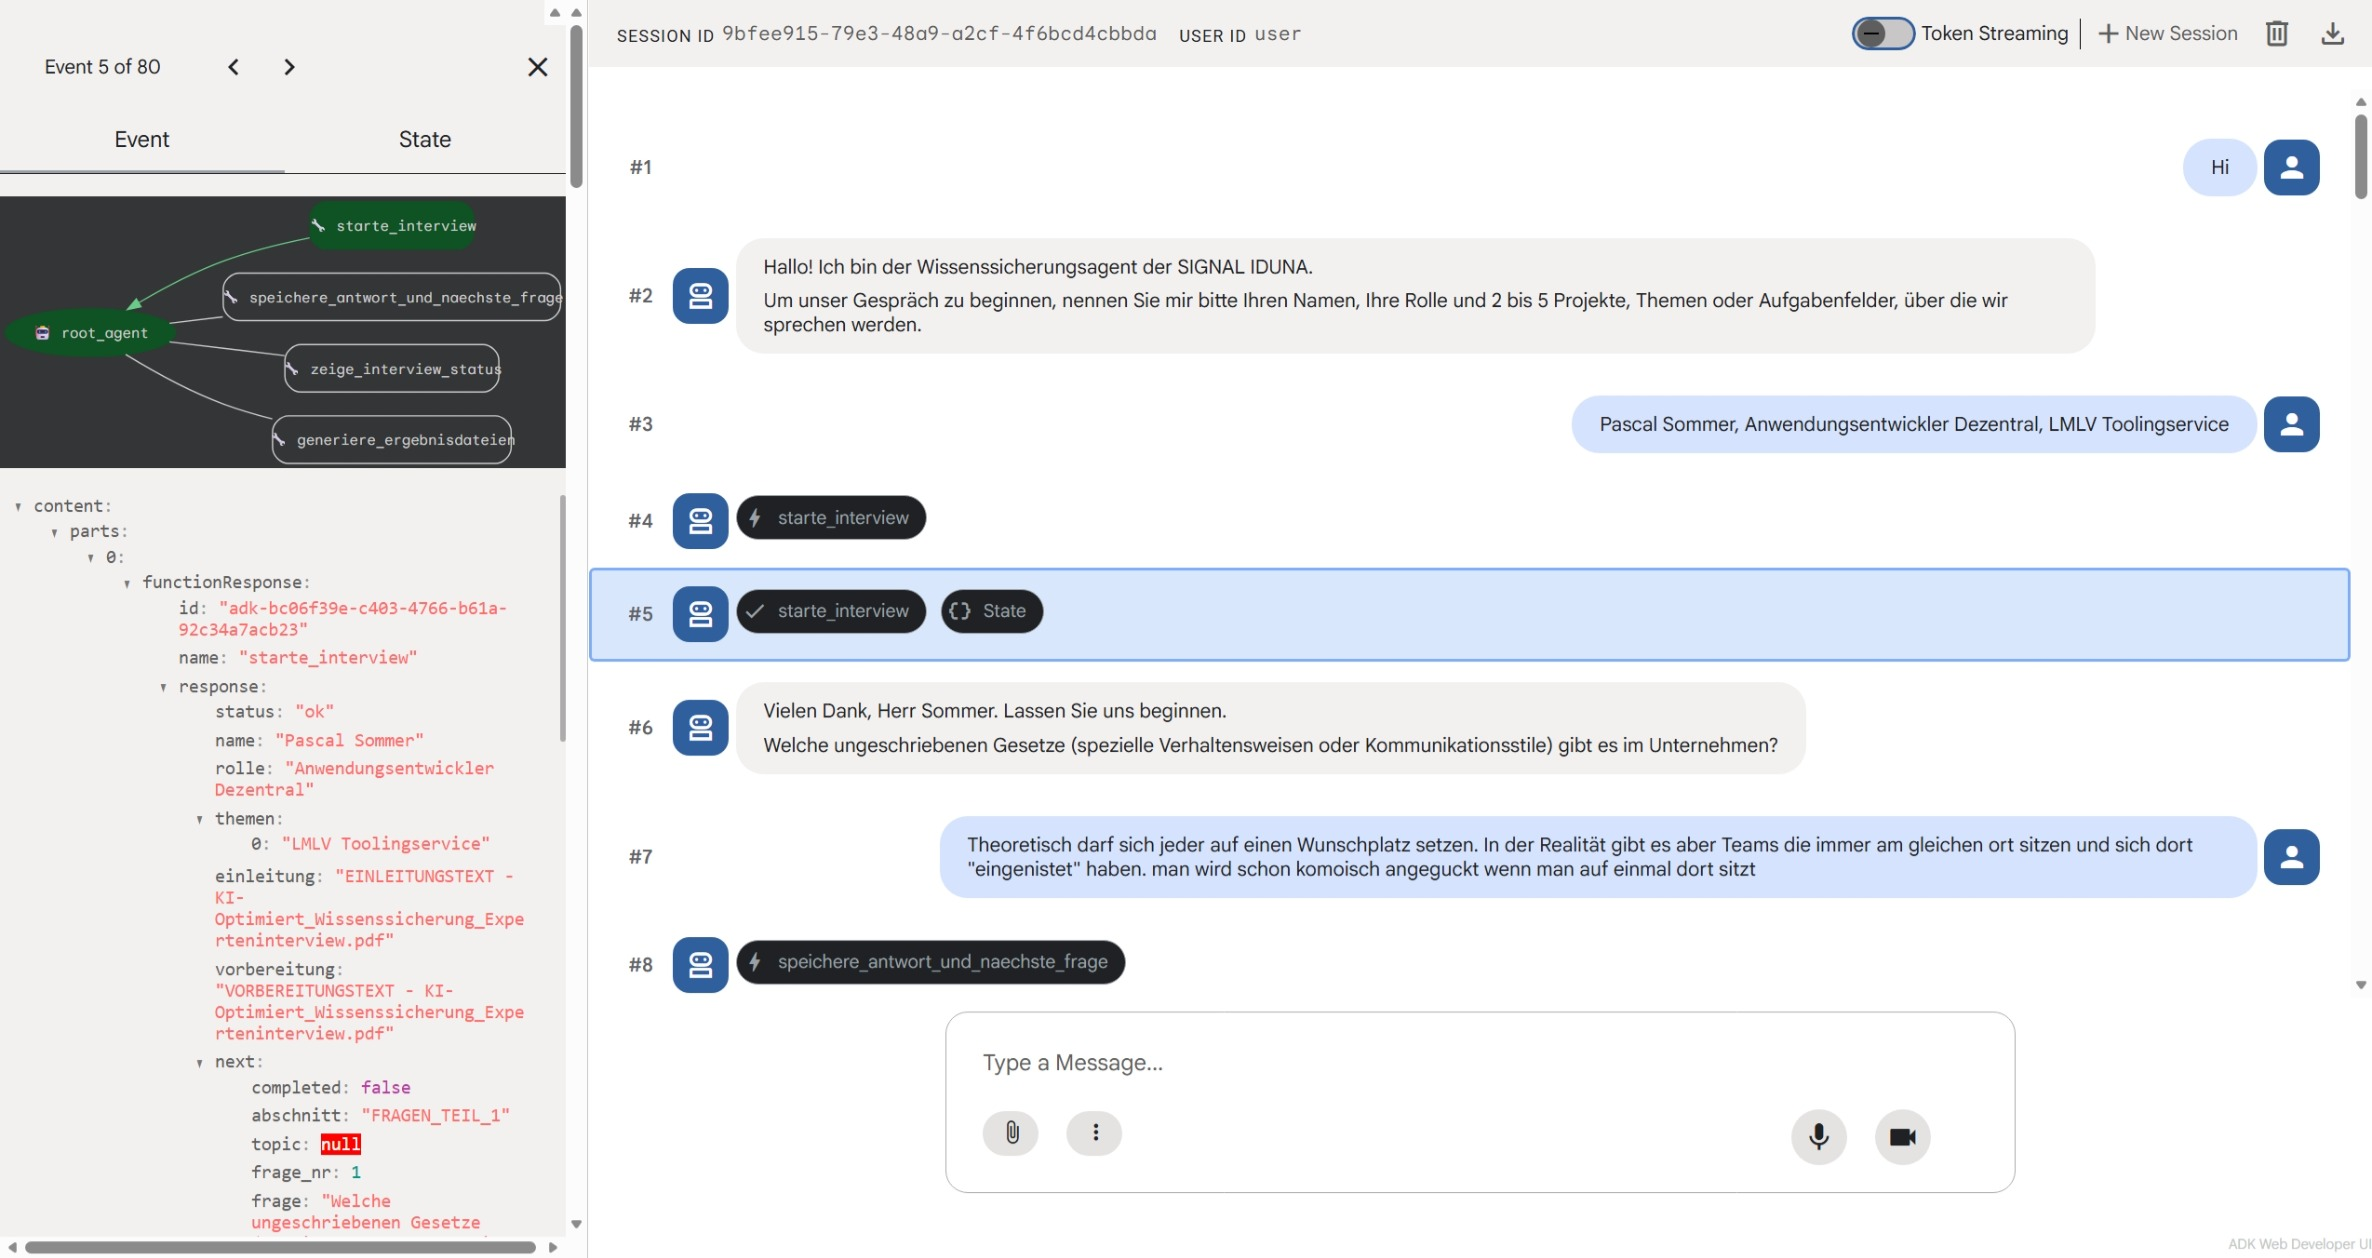
\includegraphics[
        width=0.95\textwidth,
        keepaspectratio
    ]{images/durchlauf1_start.jpeg}
    \caption{Interviewstart in der \glslink{adk}{ADK} Web \glslink{ui}{UI}}
    \label{fig:adk_web_ui_interviewstart}
\end{figure}

\begin{figure}[H]
    \centering
    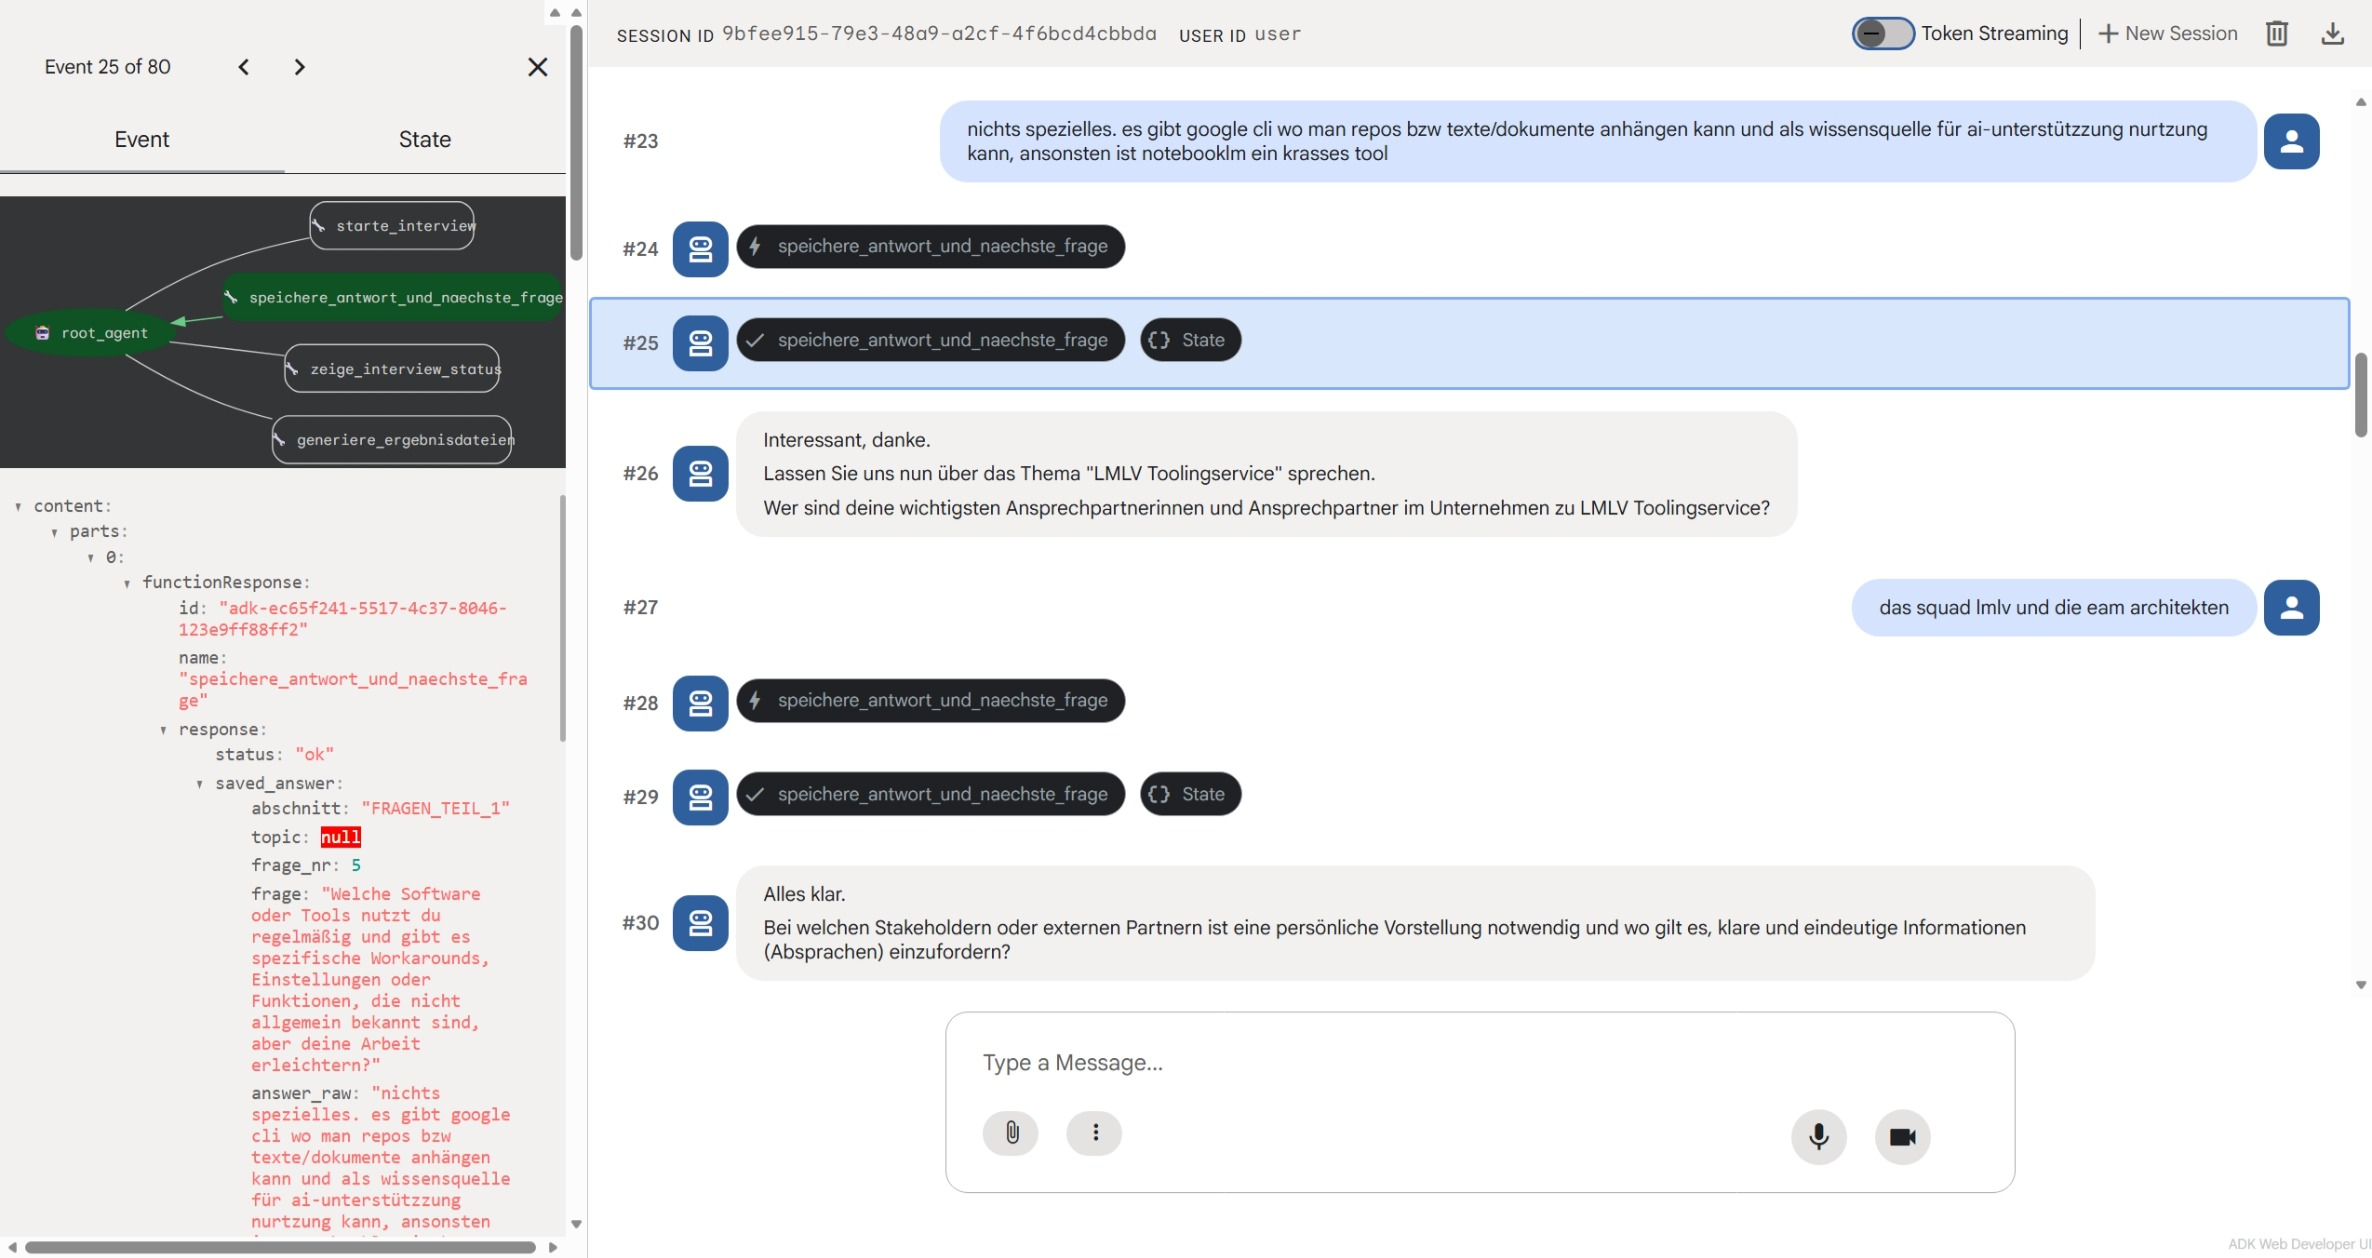
\includegraphics[
        width=0.95\textwidth,
        keepaspectratio
    ]{images/durchlauf1_switch_to_project.jpeg}
    \caption{Projektwechsel in der \glslink{adk}{ADK} Web \glslink{ui}{UI}}
    \label{fig:adk_web_ui_switch_to_project}
\end{figure}

\begin{figure}[H]
    \centering
    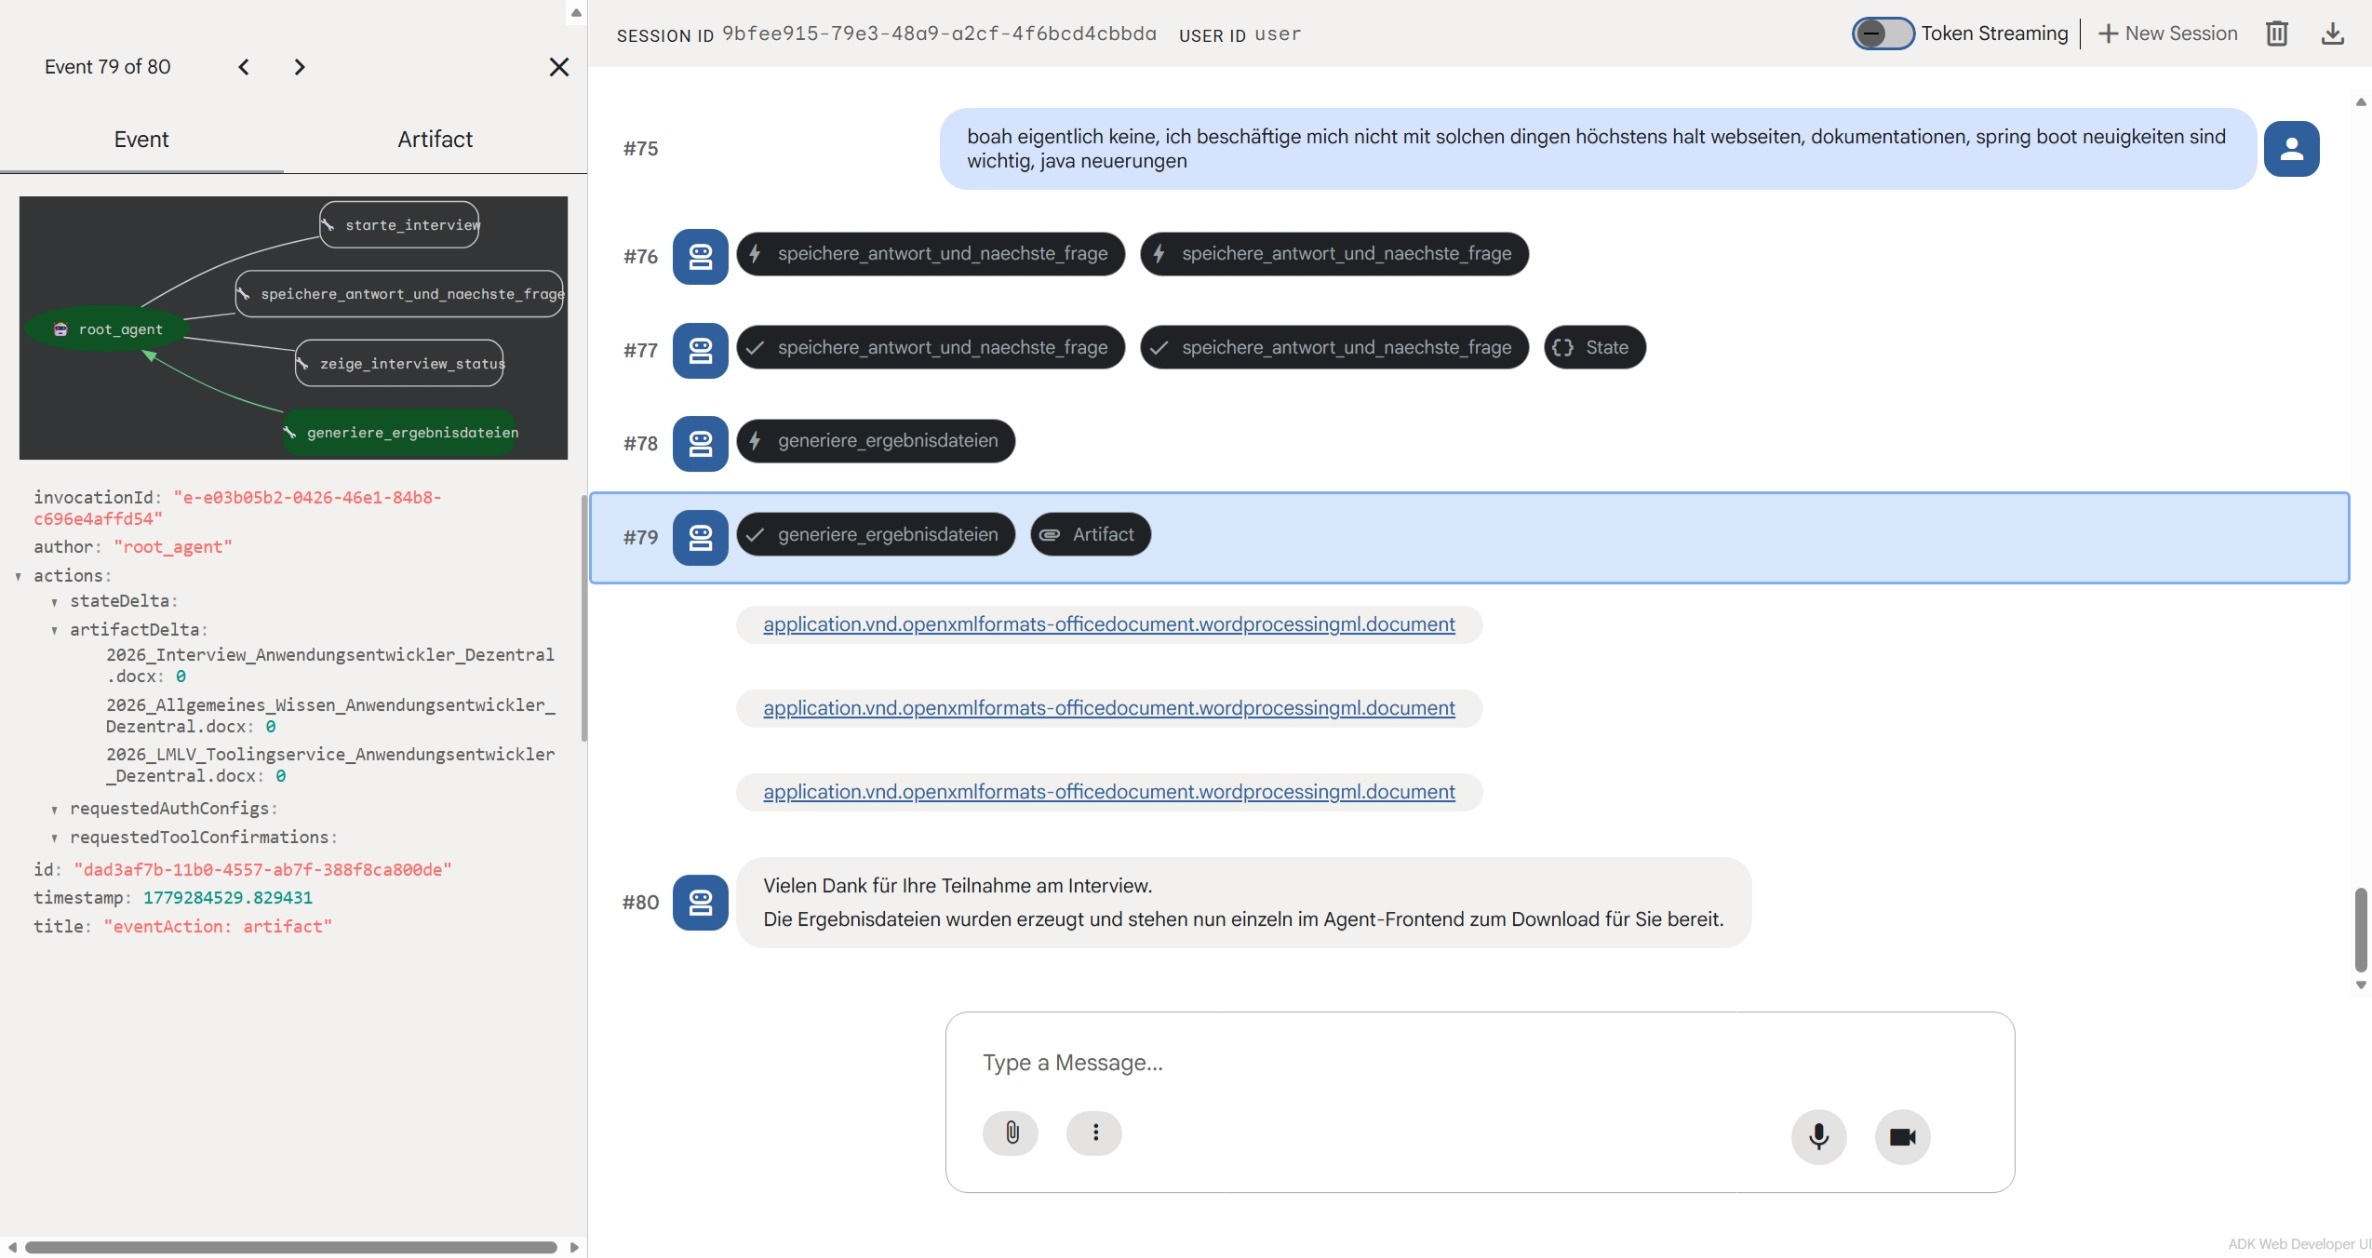
\includegraphics[
        width=0.95\textwidth,
        keepaspectratio
    ]{images/durchlauf2_dokumentenbereitstellung.jpeg}
    \caption{Dokumentenbereitstellung in der \glslink{adk}{ADK} Web \glslink{ui}{UI}}
    \label{fig:adk_web_ui_dokumentenbereitstellung}
\end{figure}
%-------------- A16 Screenshots der ADK Web UI

%Bereitstellung der Ergebnisdateien in der ADK Web UI
%-------------- A17 Fachlicher Kriterienkatalog
\newpage
\subsection{Fachlicher Kriterienkatalog}
\label{anhang_kriterienkatalog}

\begin{table}[H]
\centering
\begin{tabularx}{\textwidth}{|L{4.5cm}|Y|L{2.4cm}|}
\hline
\rowcolor{hkblue}
\textcolor{white}{\textbf{Kriterium}} 
& \textcolor{white}{\textbf{Beschreibung}} 
& \textcolor{white}{\textbf{Bewertung}} \\
\hline

\rowcolor{hklight}
Aufrufbarkeit des Agenten 
& Der Agent ist in der Testumgebung erreichbar und kann gestartet werden. 
& Nicht erfüllt \\
\hline

\rowcolor{hklight}
Nachvollziehbarer Interviewstart 
& Der Agent gibt eine Begrüßung aus, erläutert den Zweck des Interviews und beginnt mit den Eingangsfragen. 
& Erfüllt \\
\hline

\rowcolor{hklight}
Vollständiger Interviewablauf 
& Der Agent führt durch den vorgesehenen Interviewleitfaden und bietet die Pflichtfragen an. 
& Erfüllt \\
\hline

\rowcolor{hklight}
Projektbezogene Wissenssicherung 
& Der Agent stellt projekt- oder themenbezogene Fragen für angegebene Themenbereiche. 
& Erfüllt \\
\hline

\rowcolor{hklight}
Strukturierung der Antworten 
& Die Antworten werden nachvollziehbar kategorisiert und für die Ergebnisdateien aufbereitet. 
& Erfüllt \\
\hline

\rowcolor{hklight}
Bereitstellung der Ergebnisdateien 
& Die Ergebnisdateien werden erzeugt und der nutzenden Person zum Download bereitgestellt. 
& Erfüllt \\
\hline

\rowcolor{hklight}
Fachliche Nutzbarkeit 
& Der Ablauf und die erzeugten Dateien sind aus fachlicher Sicht grundsätzlich als Grundlage für die Wissenssicherung geeignet. 
& Erfüllt \\
\hline

\end{tabularx}
\caption{Fachlicher Kriterienkatalog und Abnahmebewertung}
\label{tab:kriterienkatalog_abnahme}
\end{table}
%-------------- A17 Fachlicher Kriterienkatalog

%-------------- A18 Soll-Ist-Vergleich
\newpage
\subsection{Soll-Ist-Vergleich}
\label{anhang_soll-ist-vergleich}

\begin{table}[H]
\centering
\begin{tabularx}{\textwidth}{|L{4.2cm}|Y|L{2.2cm}|}
\hline
\rowcolor{hkblue}
\textcolor{white}{\textbf{Soll-Zustand}} 
& \textcolor{white}{\textbf{Ist-Umsetzung}} 
& \textcolor{white}{\textbf{Bewertung}} \\
\hline

\rowcolor{hklight}
Aufrufbarer Agent in einer Testumgebung 
& Der Agent kann über die \gls{adk} Web \gls{ui}, jedoch nicht in einer separaten Testumgebung, gestartet und getestet werden. 
& Nicht erfüllt \\
\hline

\rowcolor{hklight}
Strukturierter Interviewablauf mit definiertem Fragenkatalog 
& Die Fragen werden aus der Discovery Engine geladen und in der vorgesehenen Reihenfolge gestellt. 
& Erfüllt \\
\hline

\rowcolor{hklight}
Wiederholung projektbezogener Fragen für angegebene Themen 
& Der zweite Fragenteil wird für jedes angegebene Projekt beziehungsweise Thema durchlaufen. 
& Erfüllt \\
\hline

\rowcolor{hklight}
Speicherung und Kategorisierung der Antworten 
& Die Antworten werden mit Frage, Rohantwort, Kurzfassung, Ergebniskategorie und Key-Word im Session State gespeichert. 
& Erfüllt \\
\hline

\rowcolor{hklight}
Erzeugung strukturierter Ergebnisdateien 
& Nach Abschluss des Interviews werden DOCX-Dokumente erzeugt.
& Erfüllt \\
\hline

\rowcolor{hklight}
Bereitstellung der Ergebnisdateien zum Download 
& Die Ergebnisdateien werden über die Artefaktfunktion der \gls{adk} Web \gls{ui} bereitgestellt. 
& Erfüllt \\
\hline

\rowcolor{hklight}
Einhaltung der \gls{mvp}-Abgrenzung 
& Produktivsetzung, automatische Ablage, Sprachschnittstelle und vollständige Konsistenzprüfung wurden nicht umgesetzt. 
& Erfüllt \\
\hline

\end{tabularx}
\caption{Soll-Ist-Vergleich des Projektergebnisses}
\label{tab:soll_ist_vergleich}
\end{table}
%-------------- A18 Soll-Ist-Vergleich

\end{document}